% Created 2022-10-20 Thu 21:56
% Intended LaTeX compiler: lualatex
\documentclass[letterpaper, 12pt]{book}
\usepackage{graphicx}
\usepackage{longtable}
\usepackage{wrapfig}
\usepackage{rotating}
\usepackage[normalem]{ulem}
\usepackage{amsmath}
\usepackage{amssymb}
\usepackage{capt-of}
\usepackage{hyperref}
\usepackage[table, dvipsnames]{xcolor}
\usepackage{listings}
\usepackage{url}
\usepackage{soul}
\usepackage{amsthm}
\usepackage{amsfonts}
\usepackage{tcolorbox}
\usepackage{graphicx}
\usepackage{wrapfig}
\usepackage{listings}
\usepackage{framed}
\usepackage{float}
\usepackage{tikz}
\definecolor{navyblue}{HTML}{000080}
\hypersetup{colorlinks=true, citecolor=RoyalBlue, linkcolor=BrickRed, urlcolor=black} % by default sets linkcolor=BrickRed, citecolor=green, filecolor=cyan, menucolor=red, runcolor=cyan, urlcolor=magenta
\usepackage{booktabs}
\usepackage{longtable}
\usepackage{array}
\usepackage{multirow}
\usepackage{hhline}
\usepackage[font=small]{caption}
\usepackage{diagbox}
\usepackage{afterpage}
\usepackage{mathtools}
\newcommand\textstyleSourceText[1]{\texttt{#1}}\makeatletter\newcommand\arraybslash{\let\\\@arraycr}\makeatother\renewcommand\arraystretch{1.3}\setlength\tabcolsep{0.01\textwidth}
\setlength{\LTpre}{20pt} \setlength{\LTpost}{-20pt}
\usepackage{enumitem}
\setlist[description]{leftmargin=0pt}
\setlist[itemize]{itemsep=0pt}
\setlist[enumerate]{noitemsep}
\theoremstyle{definition}
\newtheorem{theorem}{Theorem}[section]
\theoremstyle{definition}
\newtheorem{corollary}{Corollary}[theorem]
\theoremstyle{definition}
\newtheorem{lemma}[theorem]{Lemma}
\theoremstyle{definition}
\newtheorem{remark}{Remark}
\theoremstyle{definition}
\newtheorem{definition}[theorem]{Definition}
\lstset{language=,basicstyle=\small\ttfamily,breaklines=true,frame=single,numbers=left,morecomment=[l][\color{gray}]{//}}
\newenvironment{colbox}[1][green]{\colorlet{shadecolor}{#1!15}\begin{shaded}}{\end{shaded}}

\usepackage[left=3cm,right=3cm,top=3cm,bottom=4cm]{geometry}
\usepackage[backend=bibtex]{biblatex}
\addbibresource{../papers/thesis.bib}
\author{Partha Ghosh\\University of Tübingen}
\usepackage[parfill]{parskip}
\sethlcolor{Goldenrod}\renewcommand{\sout}{\hl}
\usepackage{fontspec}\setmainfont{Times New Roman}
\usepackage{pifont} \newcommand{\cmark}{\ding{51}} \newcommand{\xmark}{\ding{55}}
\makeatletter \newcommand\subsubsubsection{\@startsection{paragraph}{4}{\z@}{-2.5ex\@plus -1ex \@minus -.25ex}{1.25ex \@plus .25ex}{\normalfont\small\bfseries}} \newcommand\subsubsubsubsection{\@startsection{subparagraph}{5}{\z@}{-2.5ex\@plus -1ex \@minus -.25ex}{1.25ex \@plus .25ex}{\normalfont\footnotesize\bfseries}} \makeatother
\setcounter{secnumdepth}{5} \setcounter{tocdepth}{10}
\newcommand{\vth}{\boldsymbol{\theta}}
\date{}
\title{Exploring Supervised, Semi-supervised and Self-supervised Learning in Autonomous Driving}
\hypersetup{
 pdfauthor={},
 pdftitle={Exploring Supervised, Semi-supervised and Self-supervised Learning in Autonomous Driving},
 pdfkeywords={},
 pdfsubject={},
 pdfcreator={Emacs 28.2 (Org mode 9.5.5)}, 
 pdflang={English}}
\begin{document}

\maketitle


\chapter*{Abstract}
\label{sec:org6740400}
How can we learn generalized autonomous driving models for robust vision-based
 navigation in complex and dynamic settings? The status quo for solving these
 visual navigation tasks is to train visual representations and navigation
 policies with direct supervision. Along with exploring some techinques to
 improve supervised driving performance, in this work, we mainly study several
 different approaches to effectively utilize vast amounts unlabeled, highly
 diverse ego-centric navigation data that is freely available on the internet to
 robustly scale across perspectives, platforms, environmental conditions,
 scenarios, and geographical locations. We study two existing works in this
 field that employes semi-supervised and self-supervised learning, namely
 `SelfD' \cite{Zhang2022a} and `OVRL' \cite{Yadav2022}. Moreove, in this work,
 we introduce SemiD, a framework for learning scalable driving by utilizing
 large amounts of online monocular images. Our key idea is to leverage deep
 visual odometry for iterative semi-supervised training when learning imitative
 agents from unlabeled data. To handle unconstrained viewpoints, scenes, and
 camera parameters, we train an image-based model that directly learns to plan
 in the Bird’s Eye View (BEV) space. We use deep visual odometry to generate
 pseduo-labels for the the unlabeled data and augment the decision-making
 knowledge and robustness of the model via semi-supervised training. We employ a
 large dataset of publicly available YouTube videos to train SemiD and
 comprehensively analyze its generalization benefits across challenging
 navigation scenarios. Without requiring any additional data collection or
 annotation efforts, SemiD outperforms all the previous approaches and
 demonstrates consistent improvements from 51\% to 95\% in route completion and
 from 7.8\% to 13.3\% in driving score in challenging CARLA evaluation routes.

\textbf{Keywords:} Imitation Learning, Self-supervised Learning, Semi-supervised Learning

\clearpage 

\chapter*{Acknowledgements}
\label{sec:org85ffcf1}
I want to thank Bernhard Jaeger and Katrin Renz for supervising the project
and providing me with the necessary guidance and valuable support. I want to
thank Prof. Andreas Geiger for the helpful discussions. Finally, I want to
express my very profound gratitude to my parents for their continuous support
and encouragement throughout my whole life.


\clearpage 

\clearpage \tableofcontents \clearpage

\section{Introduction}
\label{sec:org1cf3344}
How should we teach autonomous systems to drive based on visual input? How can
we learn generalized models for robust vision-based navigation in complex and
dynamic settings? While humans can effortlessly transfer general navigation
knowledge across settings and platforms (e.g. geographical location, use-case,
rare-scenarios, camera mounting point), current navigation agents cannot
transfer this knowledge well. With this question in mind, we are therefore,
interested in exploring learning strategy with which navigation agents can learn
to understand, across all settings and platforms, the structure and semantics of
their environments and navigate accordingly without providing extensive direct
supervision.

The status quo for solving these visual navigation tasks is to train visual
representations and navigation policies from scratch with direct supervision.
The family of approaches that has demonstrated promising results is imitation
learning \cite{Chen2019,Codevilla2017}. The agent is given trajectories
generated by an expert driver, along with the expert's sensory input. The goal
of learning is to produce a policy that will mimic the expert’s actions given
corresponding input
\cite{article,Bojarski2016,7410669,chen2021learning,Gupta2017,Hawke2019,Li2018,Liang2018,Mueller2018,inproceedings,Osa2018,Pomerleau1988,Prakash2021,Zhang2021}.
Now, every minute, vast amount of highly diverse and freely available
ego-centric navigation data containing such scenarios are uploaded to the
web. Even though the expert's actions may not be readily available from these
demonstration data, these data can be parsed to recover the corresponding
expert's action.  Another feasible approach could be to learn better
representations from these unlabeled data which is a very popular topic in
visual recognition. The learned representations are shown to be generalizable
across visual tasks ranging from image classification, semantic segmentation, to
object detection \cite{Chen2020a,Grill2020,He2019,Caron2020,Caron2021}. However,
these methods are primarily built for learning features for recognition tasks
rather than navigation. Therefore, in this work we aim towards effectively
utilizing such freely available demonstration data to improve the efficiency,
safety, and scalability of generalized real-world navigation agents.

We explore two different type of learning in the context of self-driving that
facilitates learning from large amounts of unlabeled experience (combined with a
small amount of direct supervision): (1) Semi-supervised Learning, (2)
Self-supervised Representation Learning. Both semi-supervised and
self-supervised methods are similar in the sense that they both facilitate
learning from large amounts of unlabeled experience, but the way both formulate
this, is quite differently. In semi-supervised learning, we devise strategies to
generate reasonable pseduo-labels to the unlabeled input driving scenes so that
upon training with these pseduo-labels the network can learn better generalized
representations of these diverse driving scenes and therefore perform better in
the navigation task. On the other hand, in self-supervised learning through
different approaches (e.g. contrastive learning, entropy regulation) the network
directly learns good representation of the unlabeled inputs. We also try to
combine both of these approaches.

In this thesis, we aim to build and compare three different learning approaches
--- two of which can be catogorized as semi-supervised learning and the other
one as self-supervised learning. We incorporate and explore an existing
semi-supervised learning approach ``SelfD'' proposed by Zhang
et. al. \cite{Zhang2022a} in our autonomous driving framework. We explore in our
self-driving framework, ``OVRL'', a self-supervised learning approach proposed
by Yadav et. al. \cite{Yadav2022} which has been studied in the domain of
embodied navigation. Moreover, we propose SemiD, a new semi-supervised learning
method that outperforms the prior works in the challenging NEAT evaluation
routes \cite{Chitta2021}. Also, we propose a data cleansing and sampling
technique for effective training. We show that combining the aforementioned
technique with mild image augmentation improve the driving performance by a huge
margin.


In summary, the main contributions of this work are:
\begin{itemize}
\item We present SemiD, a novel semi-supervised learning approach based on deep
visual odometry for autonomous driving that outperforms prior works in the
challenging NEAT evaluation routes.
\item We showed that combining SemiD and OVRL brings further improvements in route
completion.
\item We propose a data cleaning pipeline and stratified sampling in training to
improve the driving perfomance.
\item We find that image augmentations is quite important for achieving good performance.
\item We show that the inertia problem can be solved by employing the above techniques.
\end{itemize}

We organize the structure of the thesis as follows. We first provide an overview
of the related works in this field in Section \ref{org3b1a534}. Then, in Section \ref{org87c7b5d}, we introduce
our autonomous driving framework where we will deploy all our learning
approaches. In Section \ref{org96f2539}, we describe in details various
semi-supervised and self-supervised learning approaches. Next, we discuss the
experiment results in Section \ref{orgb8662bc}, followed by the conclusion in Section \ref{org156c67e}.

\section{Related Work \label{org3b1a534}}
\label{sec:org182c79a}
\subsection{End-to-End Autonomous Driving}
\label{sec:org7a8a387}
End-to-End driving describes approaches in which the entire driving task is done
by a single neural network that directly maps the raw sensor data to the driving
commands. The neural network can be trained using different algorithms, the two
most important ones being imitation learning and reinforcement learning. Even
though the models are hard to interpret, the advantages of this approach is that
these models can be optimized directly for driving. Furthermore, data
annotations are cheap, since a camera can be attached to a car and sensors to
the steering mechanisms to collect data automatically. This approach was used
early on by researchers like Pomerleau et al. and their ALVINN-vehicle
\cite{Pomerleau1988} and still active research is going on in this field
\cite{Janai2020,Tampuu2020}. Imitation Learning for driving has advanced
significantly \cite{Bojarski2016,Codevilla2017,Mueller2018} and is currently
employed in several state-of-the-art approaches, some of which predict waypoints
\cite{Casas2021,Chen2019,Filos2020}, whereas others directly predict vehicular
control
\cite{Behl2020,Buehler2020,Codevilla2019,9157137,Xiao2019,Prakash2020}. While
other learning-based driving methods such as affordances
\cite{Sauer2018,Xiao2020} and reinforcement learning
\cite{chen2021learning,Toromanoff2019,Wang2020a} could also benefit from a
semi-supervised or self-supervised learning, in this work, we try to improve
imitation learning based autonomous driving through semi/self-supervised
learning.

\subsection{Imitation Learning}
\label{sec:org4707ac7}
Imitation Learning is the most promising approach for self-driving. Our main
idea is to leverage the scale and diversity of readily accessiblem online
ego-centric navigation data to learn a robust conditional imitation learning
policy \cite{Chen2019,Codevilla2017}. While learning from labeled demonstrations
can significantly simplify the challenging vision-based policy learning task
\cite{article,Bojarski2016,7410669,chen2021learning,Gupta2017,Hawke2019,Li2018,Liang2018,Mueller2018,inproceedings,Osa2018,Pomerleau1988,Prakash2021,Zhang2021,DBLP:journals/corr/abs-1912-02973,Zhou2019a},
observed images in our settings are not labeled with corresponding actions of a
demonstrator. Therefore we aim to generalize current conditional imitation
learning (CIL) approaches \cite{Chen2019,Codevilla2017,Codevilla2019} to learn,
from unlabeled image observations, an agent that can navigate in complex urban
scenarios. To address this challenging observational learning task, prior work
has recently explored introducing various restrictive assumptions, including
access to a hand-designed reward function \cite{Chang2020}, an interactive
environment for on-policy data collection \cite{torabi2018}, or demonstrator
optimality \cite{torabi2018,Torabi2019}. We instead facilitate scalable training
from diverse data sources, by employing semi-supervised or self-supervised
learning approaches. Our resulting model can also be used to bootstrap other
methods for policy training, e.g., model-based or model-free reinforcement
learning approaches \cite{chen2021learning,Liang2018,9157137,Toromanoff2019}.

\subsection{Semi-Supervised Learning for Navigation \label{org1ae921c}}
\label{sec:org468eee3}

\subsubsection{Semi-supervised Learning}
\label{sec:org23681e8}
Semi-supervised learning is an approach to machine learning that combines a
small amount of labeled data with a large amount of unlabeled data during
training. It falls between unsupervised learning (with no labeled training data)
and supervised learning (with only labeled training data). It is a special
instance of weak supervision. Semi-supervised learning more closely imitates the
way humans learn. In semi-supervised learning, the neural network learns in two
steps:

\begin{itemize}
\item \emph{Transductive Learning:} First, the task is solved based on pseudo-labels
(i.e. by labelling the given unlabelled data) which help to initialize the
network weights.
\item \emph{Inductive Learning:} The pre-trained network is then fine-tuned with the
small ground truth data.
\end{itemize}

\subsubsection{Learning by Cheating}
\label{sec:orgc656657}
The prior works \cite{Caine2021,Yang2021, Lee2013,Rizve2021}, emphasizing
semi-supervised learning through image and object-level recognition tasks, has
limited utility for complex decision-making tasks. On the other hand, CIL
involves learning to make complex actions, from known actions of
human/privileged experts \cite{Codevilla2017,Codevilla2019,Prakash2021}. This
issue has been addressed in the recent work `Learning by Cheating' (LBC) by Chen
et al. \cite{Chen2019}. LBC utilizes a multi-stage training step, where a
privileged (i.e., ‘teacher’) CIL agent is employed to provide supervision to a
non-privileged (i.e., ‘student’) visuomotor CIL agent. The privileged CIL agent
uses a semantic segmentation bird’s eye view image as input that is processed by
a ResNet and outputs waypoints that are processed by a PID controller to produce
the driving controls. The non-privileged agent uses a similar network design but
takes as input a frontal camera image, the car’s velocity and the conditional
command by the navigational planner. As the privileged agent is given access to
extensive ground truth information about the world in training and testing, it
produces highly plausible and clean trajectories, and thus helps the
non-privileged CIL agent to learn how to drive. Learning by Cheating was the
first approach to solve the original CARLA benchmark.


In contrast, our framework for learning is very different. In semi-supervised
driving with DeepVO, we generate pseduo-labels for diverse out-of-distribution
driving scenes and to enable transductive learning of the sensorimotor
agent. SelfD, on the other hand, leverages the same visuomotor architecture as
teacher and student. We also train in inherently noisy settings, as teacher
inference is performed on diverse out-of-distribution image data and not on the
original training dataset.
\subsection{Self-Supervised Visual Representation Learning \label{org4fa78d9}}
\label{sec:orgff19362}

\subsubsection{Self-supervised learning}
\label{sec:orgd727328}
Self-supervised learning (SSL) is a machine learning approach where the
supervisory signal is automatically generated. More precisely, SSL refers to
learning data representations by solving a so-called pretext (or auxiliary)
task, in a self-supervised fashion, i.e. you automatically generate the
supervised signal from the unlabelled data.

\subsubsection{Contrastive Learning}
\label{sec:orge56af60}
The core idea of contrastive learning is to attract the positive sample pairs
and repulse the negative sample pairs. This methodology has been recently
popularized for self-supervised representation learning \cite{Wu2018}. Simple
and effective instantiations of contrastive learning have been developed using
Siamese networks \cite{He2019,Chen2020a,Zbontar2021}. In practice,
contrastive learning methods benefit from a large number of negative
samples. These samples can be maintained in a memory bank \cite{Wu2018}. In a
Siamese network, MoCo \cite{He2019} maintains a queue of negative samples and
turns one branch into a momentum encoder to improve consistency of the
queue. SimCLR \cite{Chen2020a} directly uses negative samples coexisting in the
current batch, and it requires a large batch size to work well.

\subsubsection{Non-Contrastive Learning}
\label{sec:orgfd6e37a}
Recent works have shown that we can learn unsupervised features without
discriminating between images. Grill et al. \cite{Grill2020} propose a
metric-learning formulation called BYOL, where features are trained by matching
them to representations obtained with a momentum encoder. Methods inspired from
BYOL \cite{Chen2020,Caron2021}, have shown that this method works even without a
momentum encoder.

\subsubsection{Action-COnditioned Policy Pretraining (ACO)}
\label{sec:orge9ef96d}
Action-Conditioned policy pretraining paradigm, uses contrastive learning to
capture important features in the neural representation relevant to the decision
making and benefits downstream tasks. The methods, proposed by Zhang
et. al. \cite{Zhang2022} works by first collecting a large corpus of driving
videos with a wide range of weather conditions, from wet to sunny, from all
across the world without labeling and then generating action pseudo labels for
each frame using a pretrained inverse dynamics model. Then, instead of
contrasting images based on different augmented views, this method considers a new
contrastive pair conditioned on action similarity and by learning with those
action-conditioned contrastive pairs, the representation captures policy-related
elements that are highly correlated to the actions. The experimental
results show that ACO successfully learns generalizable features for the downstream task such as policy learning through Imitation Learning (IL) and Reinforcement Learning
(RL) in end-to-end autonomous driving, and Lane Detection (LD).

In contrast, we focus on non-contrastive learning, particularly, the method DINO
proposed by Caron et. al. \cite{Caron2021}, to learn visual representations from
the unlabeled data. These generic representations can then be transferred to the
policy learning task.

\section{Autonomous Driving Framework \label{org87c7b5d}}
\label{sec:org2d8c60b}
We consider the task of point-to-point navigation in an urban setting where
the goal is to complete a given route while safely reacting to other dynamic
agents and following traffic rules. To achieve this, we consider the imitation
learning approach of learning policy, as in self-driving it is easier for an
expert to demonstrate the desired behaviour rather than to specify a reward
function.

\subsection{Imitation Learning \label{orgb2e7131}}
\label{sec:org24ff038}
The goal of Imitation Learning (IL) is, for an agent to learn a policy
\(\pi_{\boldsymbol{\theta}}\), that imitates the behavior of an expert \(\pi^{*}\). The
agent learns to map an input to a navigational decision. In general, the
decision may either be a low-level vehicle control action
\cite{Codevilla2019} (e.g. steering, throttle and break) or a desired future
trajectory relative to the ego-vehicle, i.e., a set of \(K\) waypoints
\cite{Chen2019,Mueller2018} in the BEV (birds-eye-view) space. In the latter
case, future waypoints may be paired with a hand-specified or learned motion
controller to produce the low-level action \cite{Chen2019,Mueller2018}. In
this work, we focus on the later representation due to its interpretability
and genralizability. To find the mapping, we consider the Behavior Cloning
(BC) approach of IL. To explore different learning approaches in Section
\ref{org96f2539}, we would need access to small amount of ground truth
data. For that, an expert policy is first rolled out to collect at each
time-step, high-dimensional observations of the environment including front
camera image, ego-vehicle position and orientation, high-level navigational
command and high-level goal location provided as GPS coordinates etc. From
these high-dimensional observations, we derive our dataset \(\mathcal{D} = \left\lbrace (\textbf
   X_{i}, \textbf W_{i}) \right\rbrace_{i=1}^{N}\in(\mathcal{X},\mathcal{W})\) of size \(N\), where the input
\(\textbf X\) consists of the front camera image and the goal location and the
corresponding expert trajectory \(\textbf W\), defined by a set of 2D waypoints
relative to the coordinate frame of the ego-vehicle in BEV space, i.e., \(\textbf
   W=\left\lbrace \textbf w_{t}=(x_{t},y_{t}) \right\rbrace_{t=1}^{T}\), are calculated from the
ego-vehicle positions and orientations from the subsequent frames. Our goal
is to find a decision making policy i.e. a waypoint prediction function
\(\pi_{\boldsymbol{\theta}}:\mathcal{X}\to\mathcal{W}\) with learnable parameters
\(\boldsymbol{\theta}\in\mathbb{R}^{d}\). In BC, the policy \(\pi_{\boldsymbol{\theta}}\) is learned by
training a neural network in a supervised manner using the dataset, \(\mathcal{D}\),
with a loss function, \(\mathcal{L}\) i.e.  \[\underset{{\theta}}{\text{argmin }} \mathbb{E}_{(\textbf
   X,\textbf W)\sim \mathcal{D}} [\mathcal{L}(\textbf W,\pi_{\theta}(\textbf X))].\] We use the \(L_{1}\)
distance between the predicted trajectory, \(\pi_{\boldsymbol{\theta}}(\textbf X)\), and the
corresponding expert trajectory, \(\textbf W\), as the loss function. We assume
access to an inverse dynamic model \cite{10.2307/j.ctt183ph6v}, implemented
as a PID controller \(\mathbb{I}\), which performs the low-level control, i.e.,
steer, throttle and brake, provided the future trajectory \(\textbf W\). The
action are dertermined as \(\textbf A=\mathbb{I}(\textbf W)\).

\subsection{Input and Output Representations}
\label{sec:org9b13cb9}

\subsubsection{Input Representation}
\label{sec:orgcfa2320}

\subsubsubsection{Driving Scenes}
\label{sec:orgbe4fb75}
We note that, even though our collected expert demostrations from CARLA and the
YouTube driving videos are sequential, we do not use temporal data for
training. Contrary to our intuition of getting better generalization in
decision-making from sequential observations, the prior works on IL for
autonomous driving have shown that using observation histories may not lead to
performance gain \cite{Haan2019,Muller2006,Bansal2018,Wang2019a}. Thus, we use a
single time-step input. We consider the front camera with a FOV of
\(120^{\circ}\). We extract the front image at a resolution of \(960 \times 480\)
pixels which we resize and crop to \(256 \times 256\) to remove radial distortion at
the edges. Figure \ref{fig:orgbcbfbbb} shows some example driving scenes from CARLA
and the YouTube driving videos.

\afterpage{ 
\begin{center}
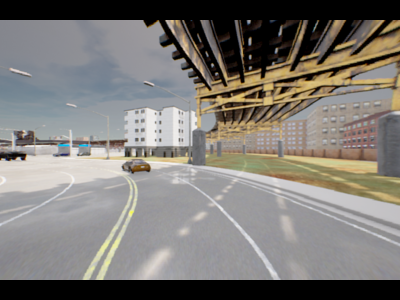
\includegraphics[trim={0 0.75cm 0 0.75cm},clip,width=0.3\textwidth]{./img/scenes/13.png}
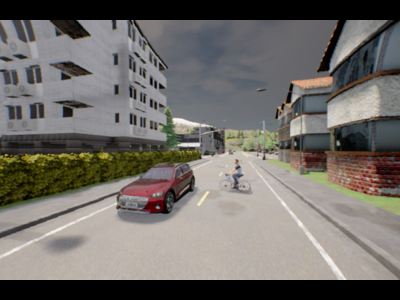
\includegraphics[trim={0 0.75cm 0 0.75cm},clip,width=0.3\textwidth]{./img/scenes/14.png}
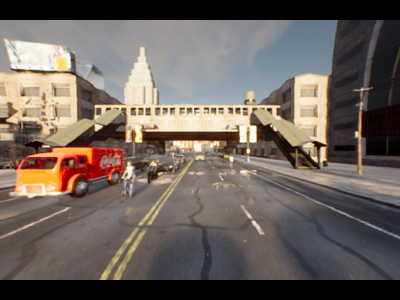
\includegraphics[trim={0 0.75cm 0 0.75cm},clip,width=0.3\textwidth]{./img/scenes/15.png}

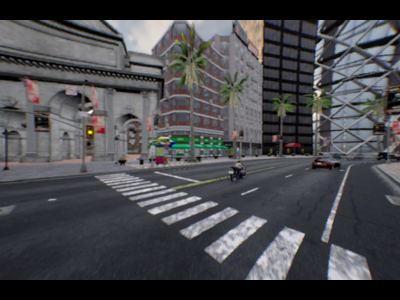
\includegraphics[trim={0 0.75cm 0 0.75cm},clip,width=0.3\textwidth]{./img/scenes/16.png}
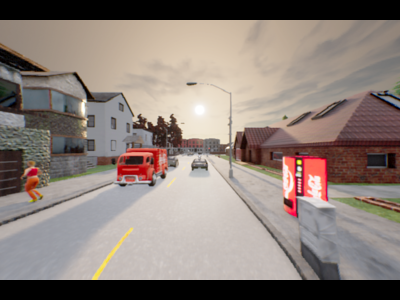
\includegraphics[trim={0 0.75cm 0 0.75cm},clip,width=0.3\textwidth]{./img/scenes/17.png}
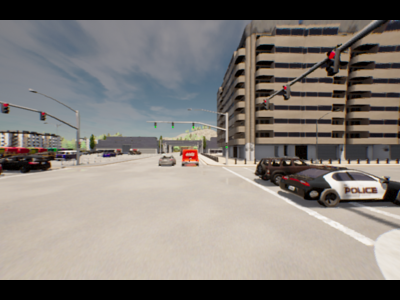
\includegraphics[trim={0 0.75cm 0 0.75cm},clip,width=0.3\textwidth]{./img/scenes/18.png}

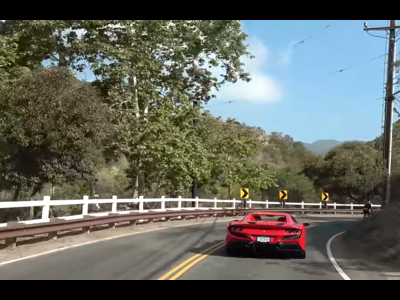
\includegraphics[trim={0 0.75cm 0 0.75cm},clip,width=0.3\textwidth]{./img/scenes/1.png}
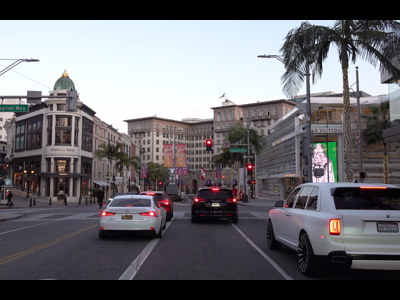
\includegraphics[trim={0 0.75cm 0 0.75cm},clip,width=0.3\textwidth]{./img/scenes/2.png}
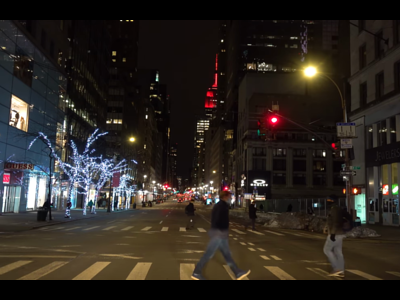
\includegraphics[trim={0 0.75cm 0 0.75cm},clip,width=0.3\textwidth]{./img/scenes/3.png}

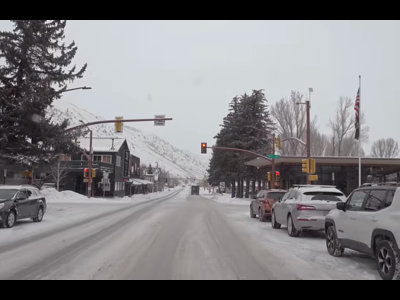
\includegraphics[trim={0 0.75cm 0 0.75cm},clip,width=0.3\textwidth]{./img/scenes/4.png}
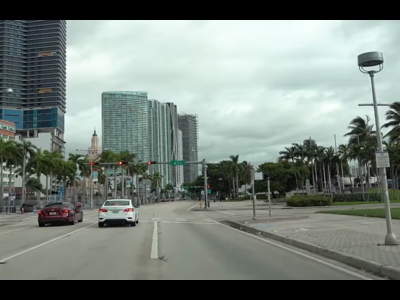
\includegraphics[trim={0 0.75cm 0 0.75cm},clip,width=0.3\textwidth]{./img/scenes/5.png}
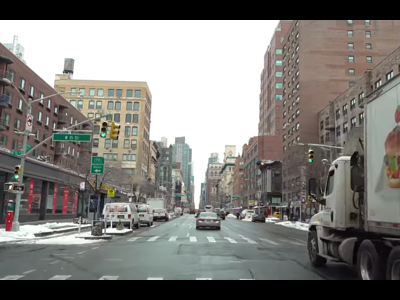
\includegraphics[trim={0 0.75cm 0 0.75cm},clip,width=0.3\textwidth]{./img/scenes/6.png}

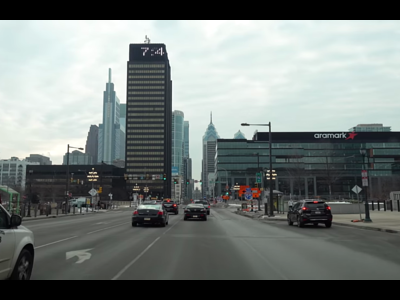
\includegraphics[trim={0 0.75cm 0 0.75cm},clip,width=0.3\textwidth]{./img/scenes/9.png}
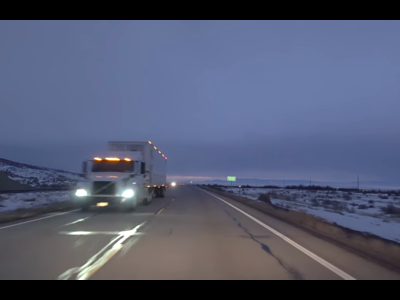
\includegraphics[trim={0 0.75cm 0 0.75cm},clip,width=0.3\textwidth]{./img/scenes/8.png}
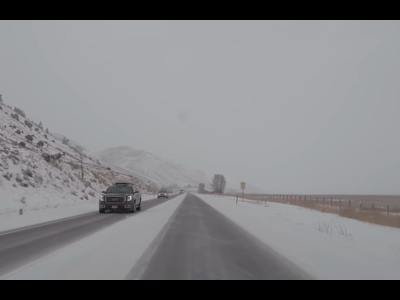
\includegraphics[trim={0 0.75cm 0 0.75cm},clip,width=0.3\textwidth]{./img/scenes/7.png}

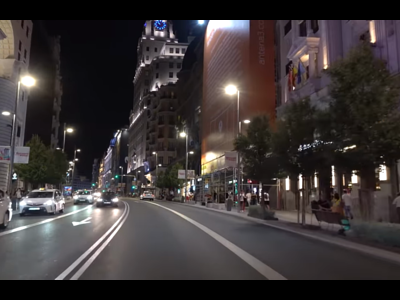
\includegraphics[trim={0 0.75cm 0 0.75cm},clip,width=0.3\textwidth]{./img/scenes/10.png}
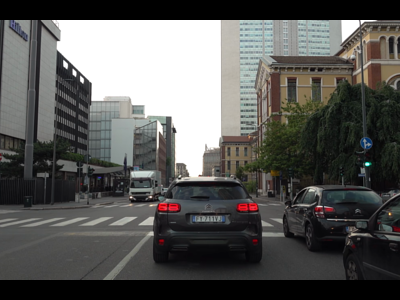
\includegraphics[trim={0 0.75cm 0 0.75cm},clip,width=0.3\textwidth]{./img/scenes/11.png}
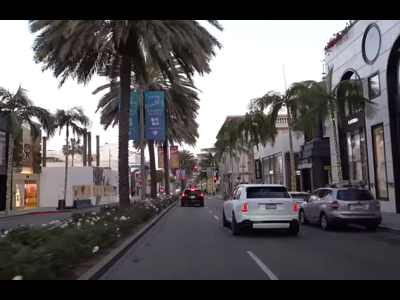
\includegraphics[trim={0 0.75cm 0 0.75cm},clip,width=0.3\textwidth]{./img/scenes/12.png}
\end{center}
\vspace{-13pt}
\begin{figure}[H]
\centering
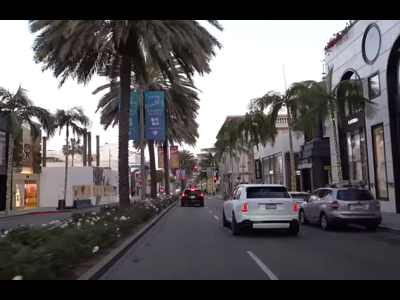
\includegraphics[height=0.01cm]{./img/scenes/12.png}
\caption{\label{fig:orgbcbfbbb}First two rows shows examples of driving scenes from the CARLA simulator and rest of the images are extracted from the YouTube driving videos.}
\end{figure}
\clearpage}


\subsubsubsection{Global Planner}
\label{sec:org0cfebb7}
We follow the standard protocol of CARLA 0.9.10 and assume that high-level goal
locations \(c\) are provided as GPS coordinates by an \(A^{*}\) navigational
planner. Agents are supposed to follow routes directed by these GPS
coordinates. Note that, these goal locations are sparse and can be hundreds of
meters apart, as opposed to the local waypoints predicted by the policy
\(\pi_{\boldsymbol{\theta}}\).

\subsubsection{Output Representation}
\label{sec:orgdd01dae}
We predict the future trajectory \(\textbf W\) of the ego-vehicle in BEV space,
centered at the current coordinate frame of the ego-vehicle. The trajectory is
represented by a sequence of 2D waypoints, \(\textbf W = \left\lbrace \textbf w_t = (x_t ,
y_t) \right\rbrace_{t=1}^{T}\).  We use \(T=4\), which is the default number of waypoints
required by our inverse dynamics model.

\subsection{Waypoint Prediction Network \label{org6328e99}}
\label{sec:orgbc2bf88}
\begin{figure}[htbp]
\centering
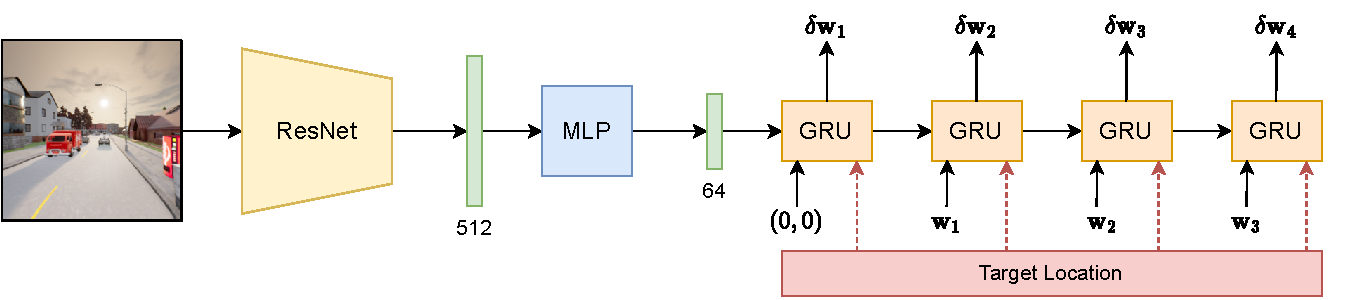
\includegraphics[keepaspectratio,width=\textwidth,height=\textheight]{./img/aim.pdf}
\caption{\label{fig:orgabe7682}Architechture of the waypoint prediction netowork AIM \cite{Prakash2021}}
\end{figure}

We adpot the image-based basline network architechture `AIM' proposed by Prakash
et. al. \cite{Prakash2021}.  As shown in Figure \ref{fig:orgabe7682}, first, we encode the input
driving scene with a ResNet34 architechture into a 512-dimensional
feature-encoding. We then pass this 512-dimensional feature vector through an
MLP (comprising 2 hidden layers with 256 and 128 units) to reduce its
dimensionality to 64 for computational efficiency before passing it to the
auto-regressive waypoint network implemented using GRUs \cite{Cho2014}. We
initialize the hidden state of the GRU with the 64-dimensional feature
vector. The update gate of the GRU controls the flow of information encoded in
the hidden state to the output and the next time-step. It also takes in the
current position and the goal location (Section \ref{orgb2e7131}) as input, which allows the
network to focus on the relevant context in the hidden state for predicting the
next waypoint.  We provide the GPS coordinates of the goal location (transformed
to the ego-vehicle coordinate frame) as input to the GRU rather than the encoder
since it lies in the same BEV space as the predicted waypoints and correlates
better with them compared to representing the goal location in the perspective
image domain \cite{Chen2019}. Following \cite{Filos2020}, we use a single layer
GRU followed by a linear layer which takes in the hidden state and predicts the
differential ego-vehicle waypoints \(\left\lbrace \delta \textbf w_{t} \right\rbrace_{t=1}^{T}\) for \(T=4\)
future time-steps in the ego-vehicle current coordinate frame. Therefore, the
predicted future waypoints are given by \(\left\lbrace \textbf w_{t}=\textbf w_{t-1} +\delta \textbf
w_{t} \right\rbrace_{t=1}^{T}\). The input to the first GRU unit is given as \((0,0)\) since
the BEV space is centered at the ego-vehicle’s position.

\subsection{PID Controller}
\label{sec:org649e8f0}
We use two PID controllers for lateral and longitudinal control to obtain steer,
throttle and brake values from the predicted waypoints, \(\left\lbrace \textbf
w_{t} \right\rbrace_{t=1}^{T}\). The longitudinal controller takes in the magnitude of a
weighted average of the vectors between waypoints of consecutive time-steps
whereas the lateral controller takes in their orientation. For the PID
controllers, we use the same configuration as in the author-provided codebase of
\cite{Chen2019}.
\subsection{Loss Function \label{org83b2fdf}}
\label{sec:org9ff27af}
We train the network using an \(L_{1}\) loss between the predicted waypoints and
the ground truth waypoints (from the expert), registered to the current
coordinate frame. Let \(\textbf w_{t}^{\text{gt}}\) represent the ground truth
waypoint for time-step \(t\), then the loss function is given by:
\[\mathcal{L}=\sum_{t=1}^{T}\left\| \textbf w_{t}-\textbf w_{t}^{\text{gt}} \right\|_{1}.\] Note that, the
ground truth waypoints \(\left\lbrace \textbf w_{t}^{\text{gt}} \right\rbrace\) which are available only at
training time are different from the sparse goal locations \(c\) provided at
both training and test time.

\section{Learning Approaches \label{org96f2539}}
\label{sec:orge1db0fe}
Our goal is to facilitate training driving policies at scale. We want to
efficiently make use of the broad and diverse experience found in large amounts
of unlabeled videos. To do so, in this section we explore a few semi-supervised
and self-supervised learning approaches. First, we introduce our proposed
semi-supervised learning method based on deep visual odometry. In the next
section, we discuss an existing semi-supervised learning approach ``SelfD''
proposed Zhang et. al. \cite{Zhang2022a} and incorporate it in our autonomous
driving framework. Lastly, we incorporate and explore in our self-driving
framework, ``OVRL'', a self-supervised learning approach proposed by Yadav
et. al. \cite{Yadav2022} which was studied in the domain of embodied navigation.

\subsection{SemiD: Semi-supervised Driving with Deep Visual Odometry \label{org0857abd}}
\label{sec:org408e00d}
In this section, we will introduce our proposed method for semi-supervised
learning for autonomous driving. Our key idea is to generate pseudo-labels for
unlabeled driving scenes by exploiting deep visual odometry, a learning-based
ego-motion estimation method, because of the following reasons:

\begin{itemize}
\item It is robust to image noise and independent of camera calibration.
\item In our expert driving dataset, the weather conditions and the time of the day
changes randomly from frame to frame. For this reason learning-based method is
a better choice for ego-motion estimation than the classical methods.
\item In our driving framework, we use a set of waypoints for low-level control and
a target point as a high-level navigational command. Intuitively, we can
understand that, for good driving performance, one requires accurately
predicted waypoints and a rough estimate of the target location. Our collected
pseduo-labels satisfies this criteria as the estimated waypoints with deep
visual odometry are fairly accurate due less error accumulation in the
beginning stages of estimation and the rough estimation of the target point is
sufficient as a high-level navigational command.
\item Visual odometry only estimate the relative motion between two frames to
recover the expert's action from the image sequence and therefore we do not
have to rely on the model's understanding of the driving.
\end{itemize}

\subsubsection{Deep Visual Odometry}
\label{sec:orga952f66}
We use an end-to-end learning approach following \cite{Wang2017, Zhai2019} to
train the model to map directly from input image pairs to an estimate of
ego-motion (in our use case, estimate relative translation is sufficient). The
model we used, is a two module Long-term Recurrent Convolutional Neural
Networks. The feature-encoding module encodes the short-term motion feature in a
pair of images, while the memory-propagating module captures the long-term
motion feature in the consecutive image pairs.

\subsubsubsection{Feature-encoding Module}
\label{sec:org59e6bf5}
In order to learn the geometric relationships from
two adjacent images, we use the following CNN architechture, inspired by
FlowNetSimple architechture \cite{Fischer2015} ignoring the decoder part of it
and only focusing the on the convolutional encoder.
\begin{table}
\begin{longtable}{r|r|r|r|r|r}
\hline
\raggedleft Layer &
\raggedleft Kernel Size &
\raggedleft Padding &
\raggedleft Stride &
\raggedleft Max Pool &
\raggedleft\arraybslash Number of Channels\\\hline
\raggedleft Input &
\raggedleft - &
\raggedleft - &
\raggedleft - &
\raggedleft - &
\raggedleft\arraybslash 6\\
\raggedleft Conv1 &
\raggedleft $3 \times 3$ &
\raggedleft 1 &
\raggedleft 0 &
\raggedleft $2 \times 2$ &
\raggedleft\arraybslash 64\\
\raggedleft Conv2 &
\raggedleft $3 \times 3$ &
\raggedleft 1 &
\raggedleft 0 &
\raggedleft $2 \times 2$ &
\raggedleft\arraybslash 128\\
\raggedleft Conv3 &
\raggedleft $3 \times 3$ &
\raggedleft 1 &
\raggedleft 0 &
\raggedleft $4 \times 4$ &
\raggedleft\arraybslash 256\\
\raggedleft Conv4 &
\raggedleft $3 \times 3$ &
\raggedleft 1 &
\raggedleft 0 &
\raggedleft $4 \times 4$ &
\raggedleft\arraybslash 512\\
\raggedleft Conv5 &
\raggedleft $3 \times 3$ &
\raggedleft 1 &
\raggedleft 0 &
\raggedleft $4 \times 4$ &
\raggedleft\arraybslash 1024\\\hline
\caption{Configuration of the CNN}
\label{table1}
\end{longtable}
\end{table}
Contrary to DeepVO \cite{Wang2017} and PoseConvGRU \cite{Zhai2019}, which uses
huge 10-layered CNN architechtures, we use a very simple and lightweight
5-layered CNN architechture as shown in Table \ref{table1}. Each layer is
followed by an application of ReLU nonlinear activation function. We keep the
kernel size to 3, padding size to 1 for all the layers. The channel dimension
doubles in each subsequent layers. We use maxpool of size 2 in the first 2
layers and use maxpool of size 4 for the rest of the layers. The reason behind
this is that, having small receptive field in the first 2 layers encourages the
network to learn about the fine-grained geometric details in the pair of images
which is essential for relative motion estimation. On the other hand, the large
receptive field in the later layers enforces the network to ignore the global
context and also helps in reducing the number of learnable parameters as
well. The input to the CNN are a sequence of \(n+1\), \(256 \times 256\) RGB driving
scenes from CARLA. With \(n+1\) sequential driving scenes, we can obtain \(n\)
sets of image pairs taking two adjacent frames at a time. These image pairs are
then fed to the 5-layered CNN to obtain a feature maps of size \(1 \times 1 \times
1024\) for each image pair. Contrary to the typical training process with
augmented data for CNNs, we only use the original images for accurate relative
motion estimation, because performing any pre-processing operation to the images
such as blurring, adding noise, random clipping etc., can hamper the network to
learn the geometric relationship of the objects in the images.

\subsubsubsection{Memory-propagating Module}
\label{sec:orgf661ae4}
Following \cite{Zhai2019}, we use a stacked GRU (Gated Recurrent Unit)
\cite{Ballas2015} as our memory-propagating module as showns in Figure \ref{fig:org8fe1c87}. The
memory module builds a set of chronological visual representations from the CNN
embeddedings of the sequence of image pairs. Because of its ability of remember
histories, GRU can capture the geometric relationships coming from the previous
frames of images, and then estimate the relative motion for the current frame
utilizing the geometric constraint within multiple frames. Also, GRUs are
appropriate for this module as they are simple yet powerful. They contain fewer
gates compared to LSTMs (Long Short-Term Memory unit) and thus reduce the number
of learnable parameters and, yet, provide similar performance as LSTMs
\cite{Chung2014}. In our implementation, we flatten the \(1 \times 1 \times
1024\)-dimensional CNN embeddeding into a feature vector, which we then further
process through a fully connected layer and reduce its dimensions to 256 for
computational efficiency before passing it to the GRU. Following
\cite{Filos2020}, we use a single layer GRU followed by a linear layer which
takes in the hidden state and predicts the relative translation of the
ego-vehicle implied by the pair of images. Finally, we accumulate all the
relative translations to compute the ego-vehicle trajectory.

\begin{figure}[H]
\centering
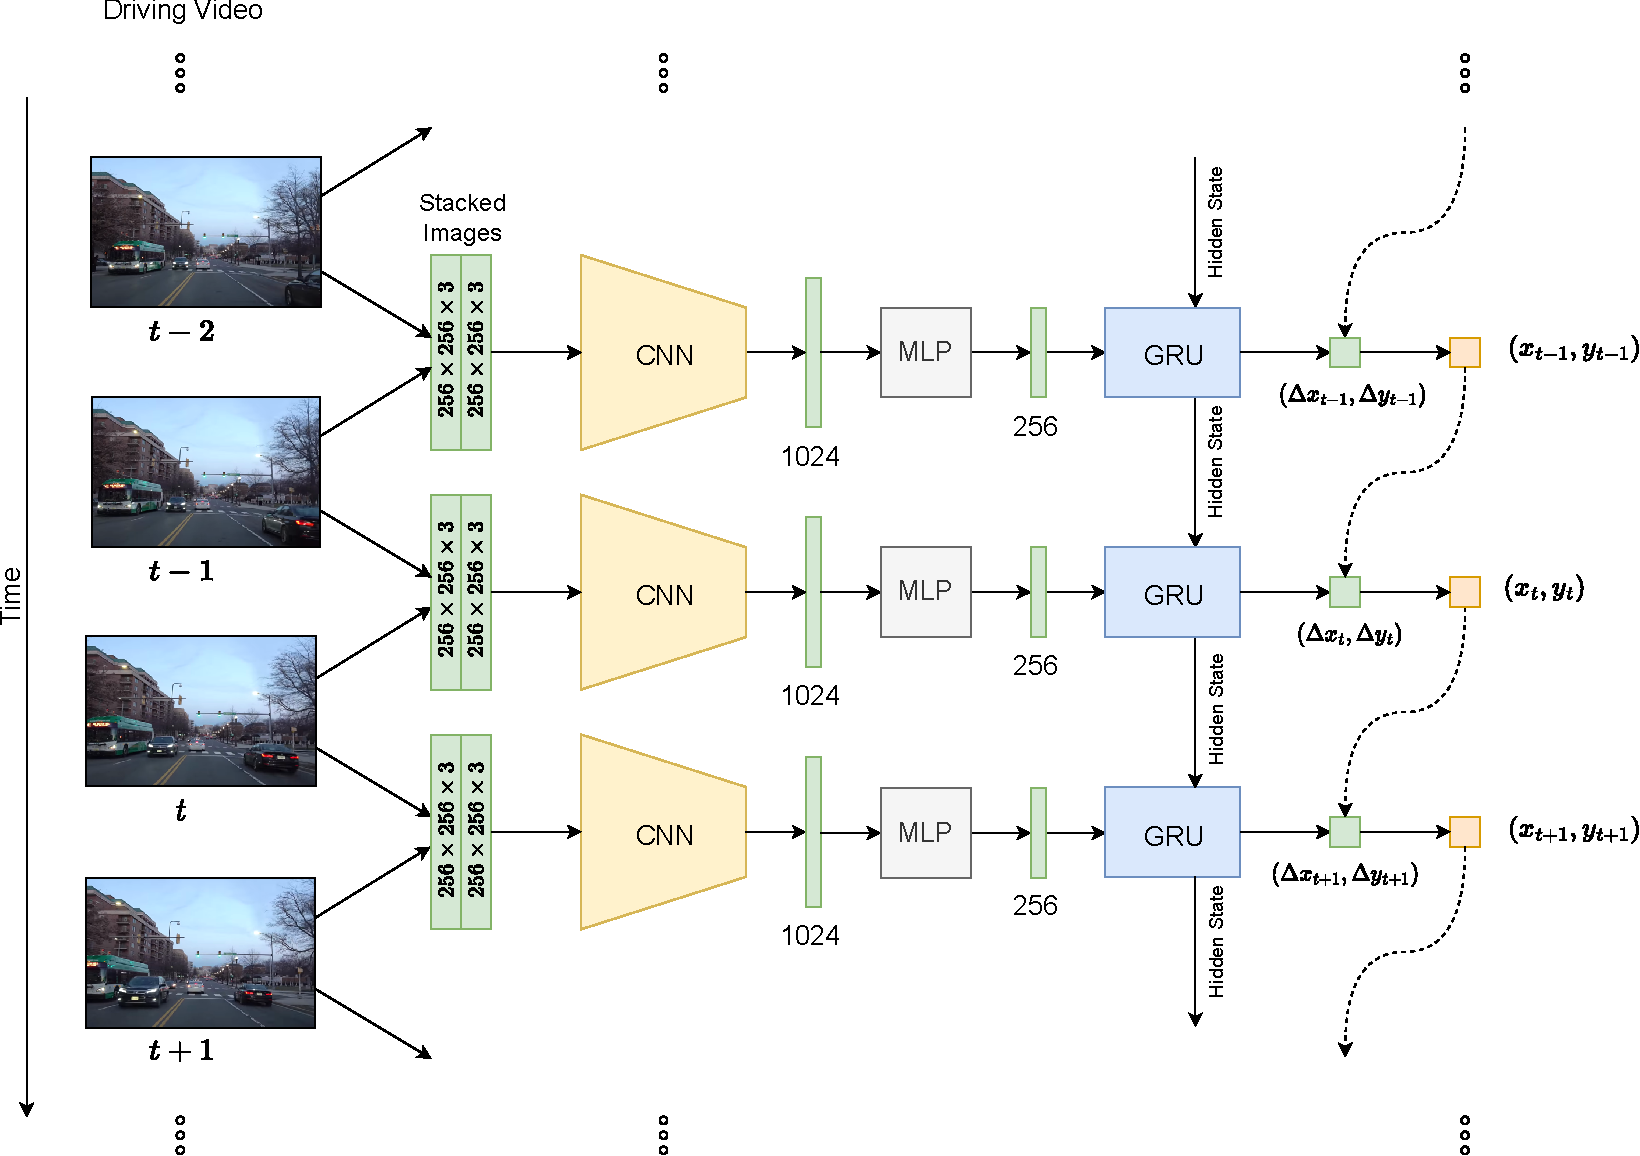
\includegraphics[keepaspectratio,width=\textwidth,height=\textheight]{./img/deepvo.pdf}
\caption{\label{fig:org8fe1c87}Architecture of the ConvGRU-based monocular VO system.}
\end{figure}

\subsubsection{Generating Pseduo-labels for Video frames}
\label{sec:org300232d}
The training of the deep visual odometry network assumes access to a small
labeled dataset \(\mathcal{D}\) (as discussed in Section \ref{orgb2e7131}), which includes driving
scenes and its corresponding ego-vehicle absolute postions, to learn the
relative motion estimation. This assumption is reasonable considering that there
are several publicly available driving datasets containing ego-vehicle position
and orientation for relative motion estimation
\cite{Geiger2012AreWR,Argoverse2}. At the inference time, we compute the
ego-vehicle trajectory with the following recursive formulation.

Let, the position and orientation of the ego-vehicle at the 0-th time-step is at
the origin of the coordinate system with its heading in the direction of the
\(x\)-axis i.e., \(x_{0}=0, y_{0}=0, \cos\theta_{0}=1, \sin\theta_{0}=0\). Then, we
can compute the ego-vehicle position and orientation at the \(t+1\)-th timestep
given its position and orientation at \(t\)-th timestep as follows:

\begin{itemize}
\item \(\Delta x_{t+1}, \Delta y_{t+1}\) be the predicted relative motion from timestep
\(t\) to \(t+1\)
\item \(\cos(\Delta\theta_{t+1}) = \frac{\Delta x_{t+1}}{\sqrt{\Delta x_{t+1}^{2}+\Delta y_{t+1}^{2}}}\)
\item \(\sin(\Delta\theta_{t+1}) = \frac{\Delta y_{t+1}}{\sqrt{\Delta x_{t+1}^{2}+\Delta y_{t+1}^{2}}}\)
\item \(\cos(\theta_{t+1}) = \cos(\theta_{t}+\Delta \theta_{t+1}) =
  \cos(\theta_{t})\cos(\Delta\theta_{t+1})-\sin(\theta_{t})\sin(\Delta\theta_{t+1})\)
\item \(\sin(\theta_{t+1}) = \sin(\theta_{t}+\Delta \theta_{t+1})=
  \sin(\theta_{t})\cos(\Delta\theta_{t+1})+\cos(\theta_{t})\sin(\Delta\theta_{t+1})\)
\item \(x_{t+1} = x_{t} + \cos(\theta_{t+1})\sqrt{\Delta x_{t+1}^{2}+\Delta y_{t+1}^{2}}\)
\item \(y_{t+1} = y_{t} + \sin(\theta_{t+1})\sqrt{\Delta x_{t+1}^{2}+\Delta y_{t+1}^{2}}\)
\end{itemize}

Now, given a sequence of driving scenes (e.g. 30), we use the above recursive
formulation and get the corresponding ego-vehicle trajectory. Now, due error
accumulation, it is evident that as we progressively aggregate more and more
relative ego-motions over a longer time horizon, the estimated trajectory
gradually drifts from the ground truth trajectory. But for our use case, we only
need accurate trajectory estimation for the first 4 steps (as we use 4 waypoints
for low-level vehicle control) which holds true due to less error accumulation
in the initial few steps. Also, a rough understanding of the target location is
sufficient for driving and so, we take the end point of the trajectory as an
estimate of the target point. Thus, we generate pseduo-labels
i.e. pseudo-waypoints and pseduo-target-point for the initial driving scene. We
repeat this procedure for all the unlabeled driving scenes and thus we create
our pseduo-labeled dataset \(\hat{\mathcal{D}}_{\text{SemiD}}\). Figure \ref{fig:org8dc9221}
illustrates some example driving scenes from CARLA and YouTube videos and their
corresponding pseduo-waypoints estimated by deep visual odometry.

\afterpage{\vspace*{\fill} 
\begin{center}
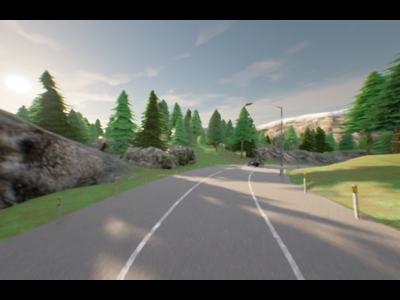
\includegraphics[trim={1.5cm 0.75cm 1.5cm 0.75cm},clip,height=0.19\textwidth]{./img/deepvo_wp/1.png}
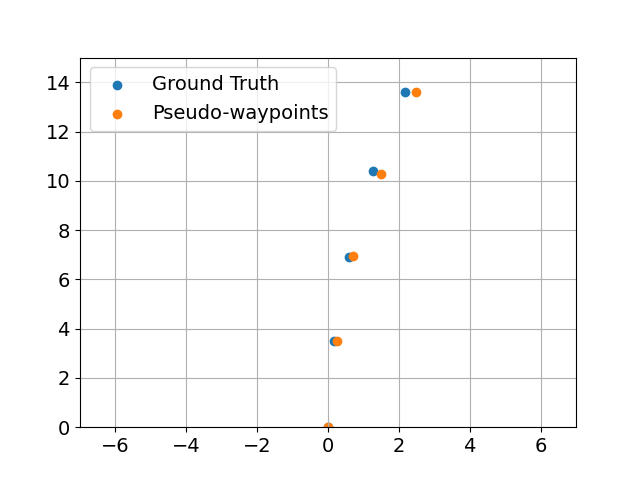
\includegraphics[trim={1cm 0.5cm 1.5cm 1cm},clip,height=0.19\textwidth]{./img/deepvo_wp/1_wp.png}
\hfill
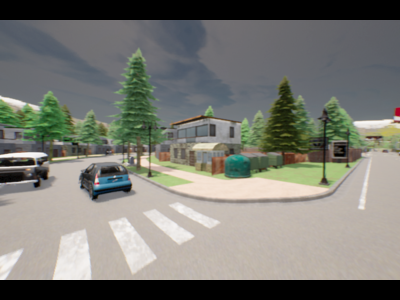
\includegraphics[trim={1.5cm 0.75cm 1.5cm 0.75cm},clip,height=0.19\textwidth]{./img/deepvo_wp/4.png}
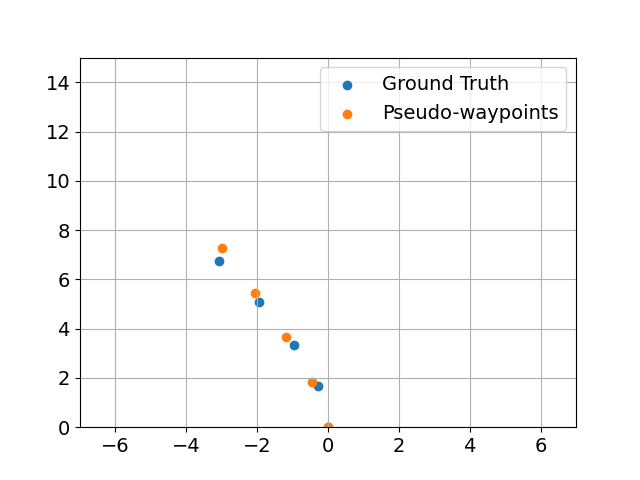
\includegraphics[trim={1cm 0.5cm 1.5cm 1cm},clip,height=0.19\textwidth]{./img/deepvo_wp/4_wp.png}

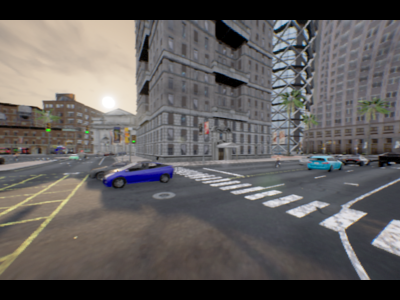
\includegraphics[trim={1.5cm 0.75cm 1.5cm 0.75cm},clip,height=0.19\textwidth]{./img/deepvo_wp/5.png}
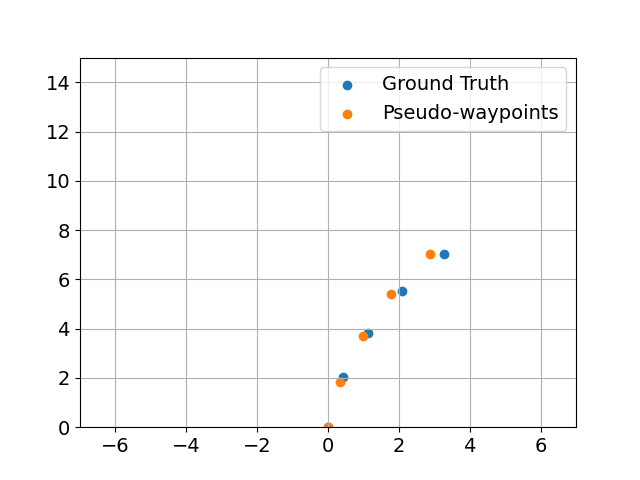
\includegraphics[trim={1cm 0.5cm 1.5cm 1cm},clip,height=0.19\textwidth]{./img/deepvo_wp/5_wp.png}
\hfill
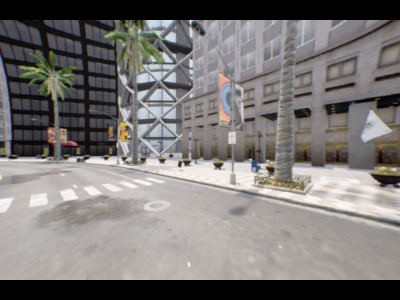
\includegraphics[trim={1.5cm 0.75cm 1.5cm 0.75cm},clip,height=0.19\textwidth]{./img/deepvo_wp/6.png}
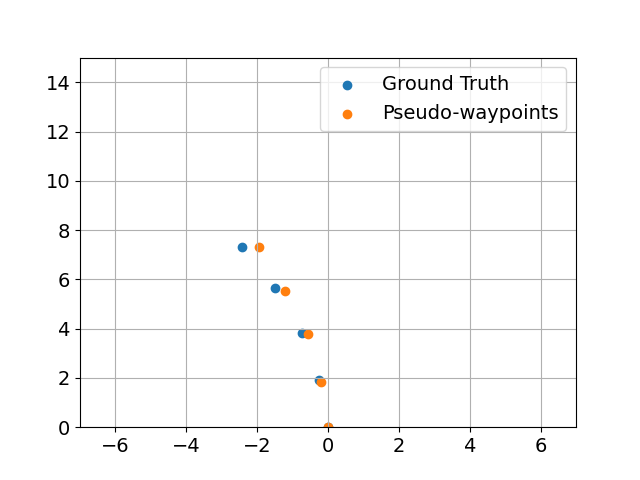
\includegraphics[trim={1cm 0.5cm 1.5cm 1cm},clip,height=0.19\textwidth]{./img/deepvo_wp/6_wp.png}

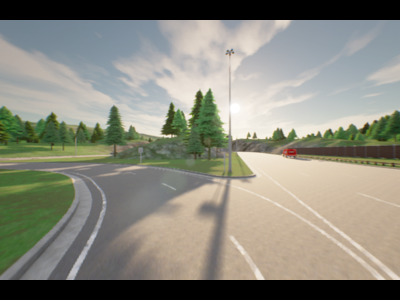
\includegraphics[trim={1.5cm 0.75cm 1.5cm 0.75cm},clip,height=0.19\textwidth]{./img/deepvo_wp/12.png}
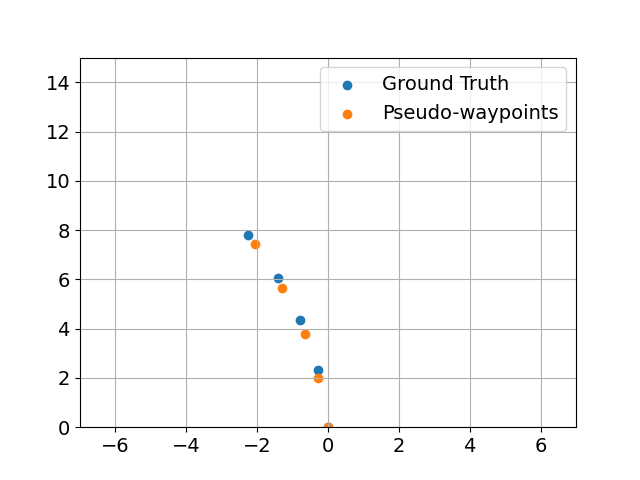
\includegraphics[trim={1cm 0.5cm 1.5cm 1cm},clip,height=0.19\textwidth]{./img/deepvo_wp/12_wp.png}
\hfill
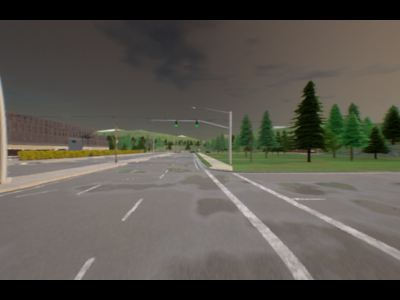
\includegraphics[trim={1.5cm 0.75cm 1.5cm 0.75cm},clip,height=0.19\textwidth]{./img/deepvo_wp/11.png}
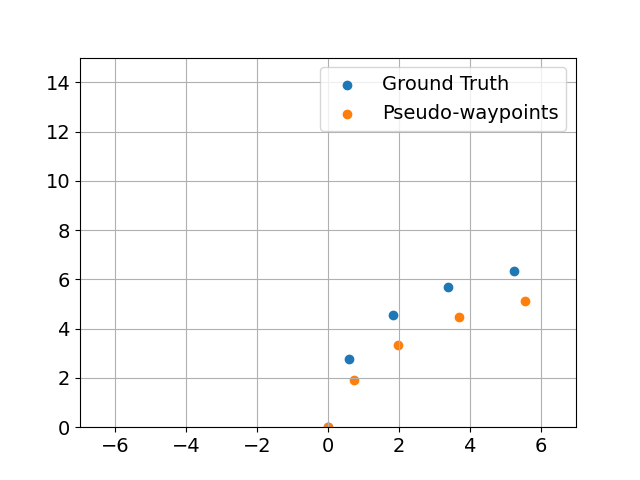
\includegraphics[trim={1cm 0.5cm 1.5cm 1cm},clip,height=0.19\textwidth]{./img/deepvo_wp/11_wp.png}

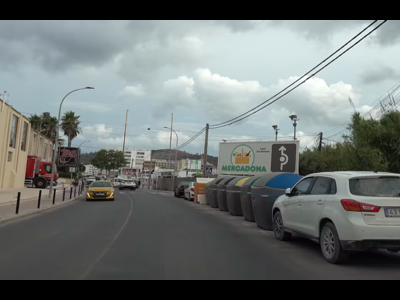
\includegraphics[trim={1.5cm 0.75cm 1.5cm 0.75cm},clip,height=0.19\textwidth]{./img/deepvo_wp/7.png}
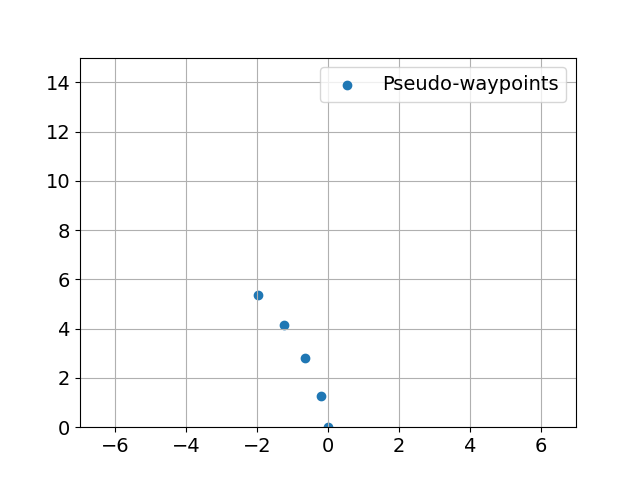
\includegraphics[trim={1cm 0.5cm 1.5cm 1cm},clip,height=0.19\textwidth]{./img/deepvo_wp/7_wp.png}
\hfill
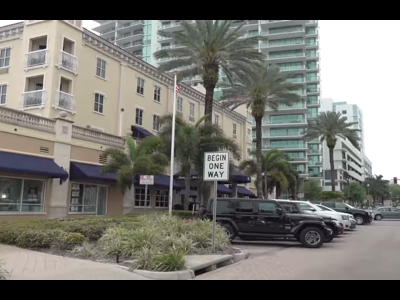
\includegraphics[trim={1.5cm 0.75cm 1.5cm 0.75cm},clip,height=0.19\textwidth]{./img/deepvo_wp/8.png}
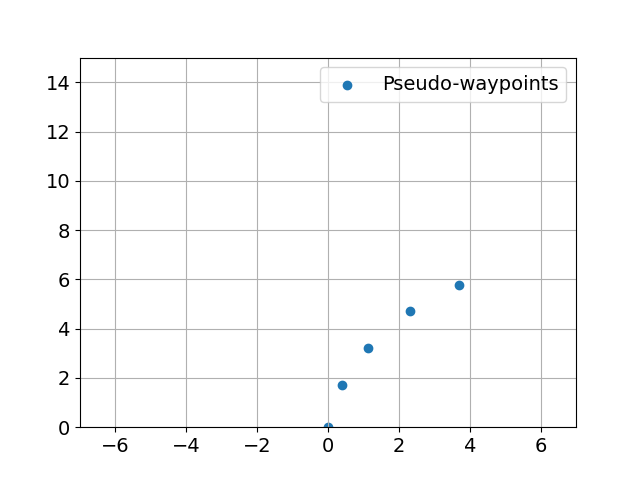
\includegraphics[trim={1cm 0.5cm 1.5cm 1cm},clip,height=0.19\textwidth]{./img/deepvo_wp/8_wp.png}

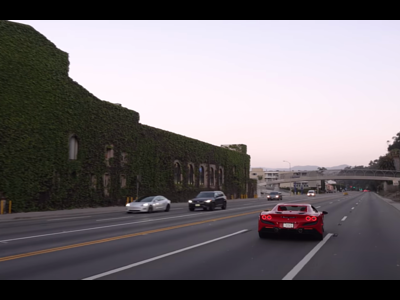
\includegraphics[trim={1.5cm 0.75cm 1.5cm 0.75cm},clip,height=0.19\textwidth]{./img/deepvo_wp/9.png}
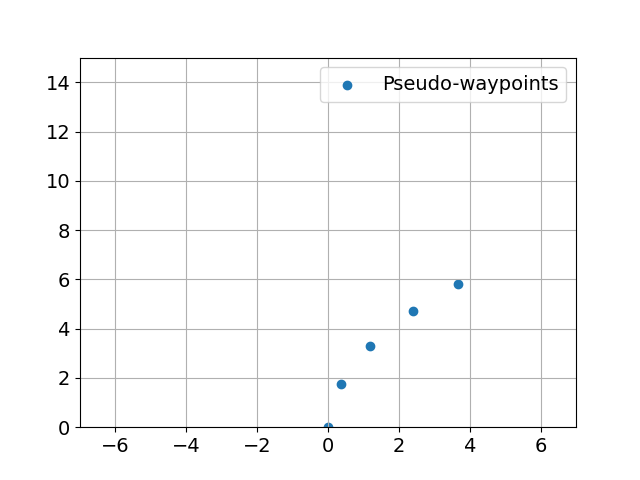
\includegraphics[trim={1cm 0.5cm 1.5cm 1cm},clip,height=0.19\textwidth]{./img/deepvo_wp/9_wp.png}
\hfill
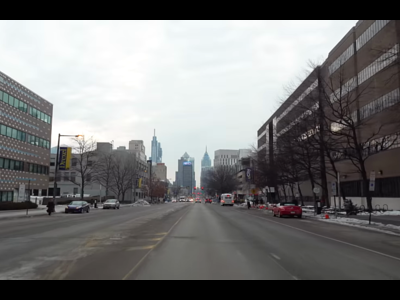
\includegraphics[trim={1.5cm 0.75cm 1.5cm 0.75cm},clip,height=0.19\textwidth]{./img/deepvo_wp/10.png}
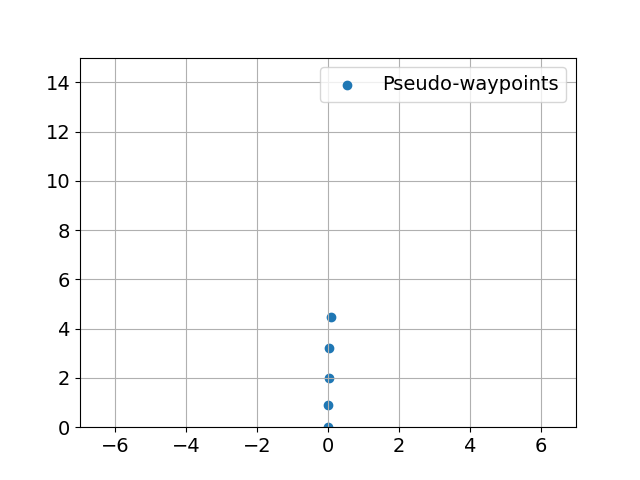
\includegraphics[trim={1cm 0.5cm 1.5cm 1cm},clip,height=0.19\textwidth]{./img/deepvo_wp/10_wp.png}
\end{center}
\vspace{-13pt}
\begin{figure}[H]
\centering
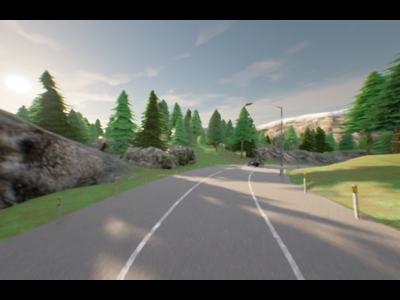
\includegraphics[height=0.01cm]{./img/deepvo_wp/1.png}
\caption{\label{fig:org8dc9221}The first three rows shows examples of driving scenes from the CARLA simulator and its corresponding ground-truth waypoints and the pseduo-waypoints estimated by the DeepVO method. The later two rows shows the estimated pseduo-waypoints of some images extracted from the YouTube driving videos.}
\end{figure}
\vspace*{\fill}\clearpage}

\subsubsection{Model Pre-Training and Fine-Tuning}
\label{sec:org7dac08b}

We pretrain the waypoint network \(\pi_{\vth}\) from scratch over the large and
diverse pseduo-labeled dataset \(\hat{\mathcal{D}}_{\text{SemiD}}\). The pre-trained policy
can then be further fine-tuned over the small original dataset \(\mathcal{D}\). Thus, we
leverage these noisy but acceptable informations from the pseduo-labeled dataset
\(\hat{\mathcal{D}}_{\text{SemiD}}\) to help the network gain a overall knowledge about the
mapping and then we provide the network with the accurate informations through
our small original dataset \(\mathcal{D}\) to enable the network to learn the mapping
from the ground-truth information.

\subsection{SelfD: Self-Learning Large-Scale Driving Policies}
\label{sec:orge69b40f}
In this section, we discuss the semi-supervised approach ``SelfD'' proposed
by Zhang et al. \cite{Zhang2022a}. We follow the three main steps. We use a
monocular image-based waypoint network AIM (Section \ref{org6328e99}) that reasons
directly in the BEV. Next, we look into the proposed data augmentation step
for obtaining multiple plausible pseudo-labels when self-training over
unlabeled YouTube data (Section \ref{org9cab8c4}). Finally, we re-train the model
over the larger dataset (Section \ref{org602bc6f}).

\subsubsection{Conditional Imitation Learning from Observations}
\label{sec:org5b18c05}
To make use of the unlabeled driving scenes containing diverse navigational
experience, the authors propose `Conditional Imitation Learning from
Observations' (CILfO) \cite{Zhang2022a} framework. The framework suggests a way
to generate pseudo-labels for the unlabeled driving scenes. But, the network
architechture used by the authors is similar to that of LBC \cite{Chen2019}
(uses discrete navigational command as the conditional command). In the work of
Prakash et. al. \cite{Prakash2021}, the authors have shown that, their proposed
image-based architechture, AIM (uses sparse goal location as the conditional
command), performs significantly better than the LBC architechture. Therefore,
in this work, we explore the CILfO framework in our autonomous driving setting
which uses AIM in its core (Section \ref{org6328e99}). Therefore, we consider sparse goal
location as the conditional command instead of the discrete navigational
commands. Therefore, utilizing the CILfO framework, we can then recover the
waypoints \(\hat{\textbf W}\), and the goal location \(\hat{c}\) from the input
image to construct a dataset \[\hat{\mathcal{D}}_{\text{SelfD}}=\left\lbrace \left( (\textbf I_{i}, \hat
c_{i}), \hat{\textbf W}_{i} \right) \right\rbrace_{i=1}^{M}\] which can be then used to train a policy
using behaviour cloning.
\subsubsection{Initial Data Assumption}
\label{sec:org04ec2f7}
The CILfO learning task assumes access to a small labeled dataset to learn an
initial policy mapping using human expert demonstrations. We then use this
learned policy to gather pseduo-labels for the unlabeled data. This assumption
is reasonable considering that there are several publicly available driving
datasets with included action labels \cite{Geiger2012AreWR,Argoverse2}. In this
work, we use the small subset of a labeled dataset \(\mathcal{D}\) collected by running
an expert policy roll out in CARLA \cite{Dosovitskiy2017} as discussed in
Section \ref{orgb2e7131}.

\subsubsection{Self-supervised Training Process}
\label{sec:orge5d1772}
In this section, we discuss the proposed generalized training method for
leveraging unconstrained and unlabeled demonstration data. The proposed
semi-supervised policy training process, SelfD, can be learned in three
summarized steps:
\begin{enumerate}
\item Use a small, labeled domain-specific dataset \(\mathcal{D}\) to learn an initial
observations-to-BEV policy \(\pi_{\boldsymbol{\theta}}\) via imitation learning.
\item Obtain a large pseudo-labeled dataset \(\hat{\mathcal{D}}_{\text{SelfD}}\) by
leveraging sampling from \(\pi_{\boldsymbol{\theta}}\).
\item Pre-train a generalized policy \(\pi_{\boldsymbol{\theta}}\) on
\(\hat{\mathcal{D}}_{\text{SelfD}}\) and fine-tune on the clean labels of \(\mathcal{D}\).
\end{enumerate}

\subsubsection{BEV Plan Network}
\label{sec:orgf2d6dd1}
To account for arbitrary cameras, viewpoints and scene layouts, the authors
proposed a monocular planner that predicts the waypoints in the image plane and
then uses a MLP to transform those waypoints in the BEV-space. In our work,
instead of proposed method, we use an equivalent alternative. We use a GRU to
predict a future plan parameterized by waypoints, directly in the BEV plan space
as discussed in Section \ref{org6328e99}. Besides using two output nodes for predicting the
waypoints, we also add one extra output node to train the augmented network to
predict the quality estimates \(\sigma\in [0,1]\) of the waypoints. We use the IOU
of the bounding boxes of the ground-truth and the predicted waypoints as a proxy
for the quality estimates of the waypoints. Therefore, our training loss
function is defined as \[\mathcal{L}=\mathcal{L}_{\text{waypoints}}+\mathcal{L}_{\text{quality}}\] where
\(\mathcal{L}_{\text{waypoints}}\) is the \(L_{1}\) distance between the ground-truth and
the predicted waypoints as discussed in \ref{org83b2fdf} and \(\mathcal{L}_{\text{quality}}\) is a
binary cross-entropy loss.

\subsubsection{``What If'' Pseudo-Labeling of the Unlabeled Data \label{org9cab8c4}}
\label{sec:orgf63b015}
Given a set of unlabeled images \(\mathcal{U}\), we sample from the trained conditional
policy \(\pi_{\vth}\) in a semi-supervised training process. Contrary to our
proposed method in Section \ref{org0857abd}, the authors do not consider visual odometry
techniques \cite{Wang2017} to recover the expert's actions, as they found these
result in highly noisy trajectories in their online video settings. Thus, they
propose to leverage a single-frame pseudo-labeling mechanism i.e. to employ the
conditional model \(\pi_{\vth}\) to generate multiple hypothetical future
trajectories in a process referred to as ``what if'' augmentation. Beyond
resolving the missing target point, the proposed augmentation claims to provides
additional supervision, i.e., a conditional agent that better reasons on what it
might need to do, for instance, if it had to turn left instead of right at an
intersection (Figure \ref{fig:org01a4bfb}). The procedure to gather ``what if''
augmentation is as follows:

\begin{itemize}
\item sample the target point \(\hat c\) uniformly from a half disk of radius 50 meters.
\item use the conditional model to gather pseudo-labels \((\hat{\textbf W},\hat \sigma) =
  \pi_{\vth}(I,\hat c)\).
\item discard noisy trajectories with some thresholding on the quality estimate
\(\hat \sigma\) and take the rest to form the pseduo-labeled dataset
\(\hat{\mathcal{D}}_{\text{SelfD}}\).
\end{itemize}
\begin{minipage}{\textwidth} 
\begin{center}
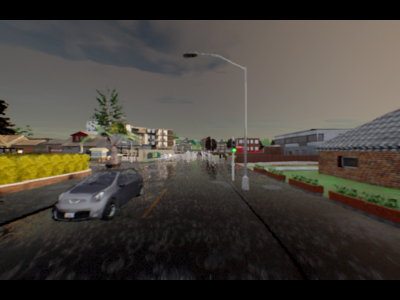
\includegraphics[trim={1.5cm 0.75cm 1.5cm 0.75cm},clip,height=0.19\textwidth]{./img/what_if/1.png}
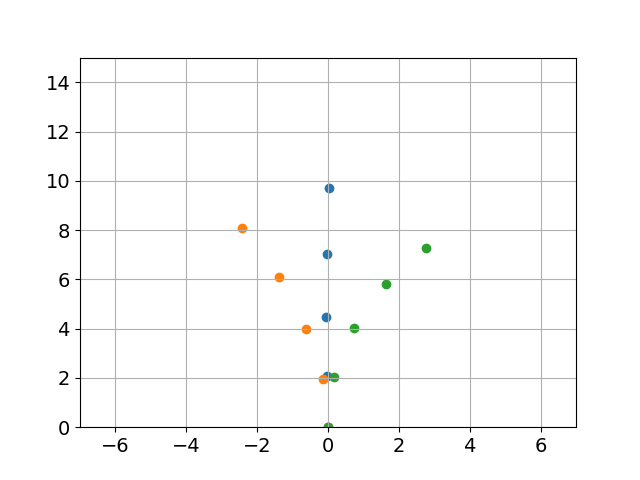
\includegraphics[trim={1cm 0.5cm 1.5cm 1cm},clip,height=0.19\textwidth]{./img/what_if/1_wp.png}
\hfill
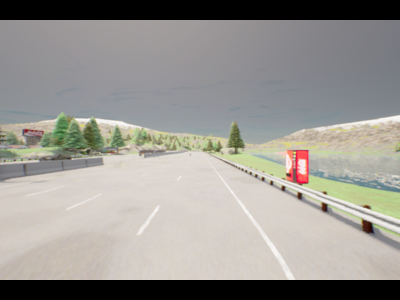
\includegraphics[trim={1.5cm 0.75cm 1.5cm 0.75cm},clip,height=0.19\textwidth]{./img/what_if/2.png}
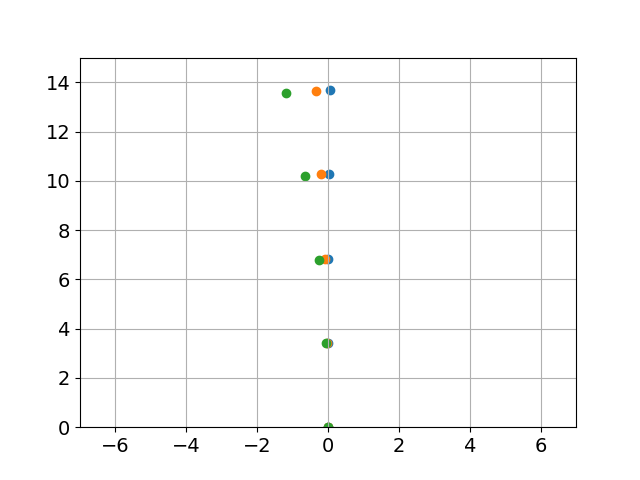
\includegraphics[trim={1cm 0.5cm 1.5cm 1cm},clip,height=0.19\textwidth]{./img/what_if/2_wp.png}

\vspace{10pt}

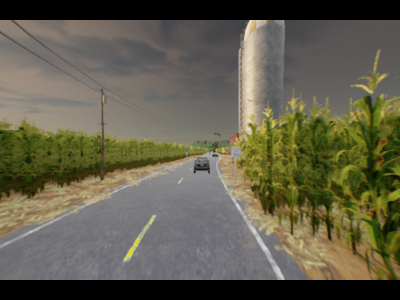
\includegraphics[trim={1.5cm 0.75cm 1.5cm 0.75cm},clip,height=0.19\textwidth]{./img/what_if/3.png}
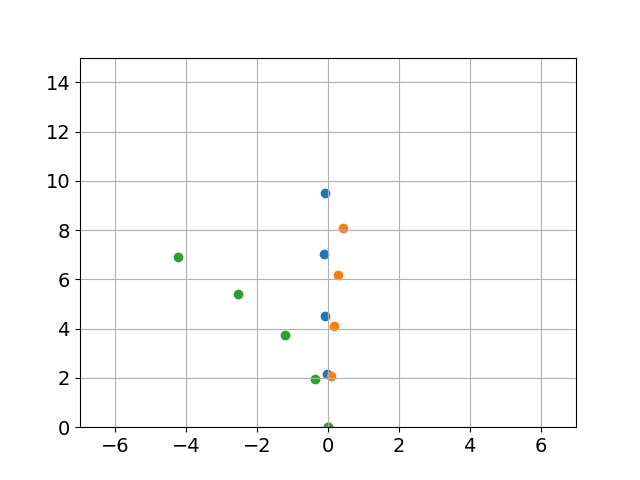
\includegraphics[trim={1cm 0.5cm 1.5cm 1cm},clip,height=0.19\textwidth]{./img/what_if/3_wp.png}
\hfill
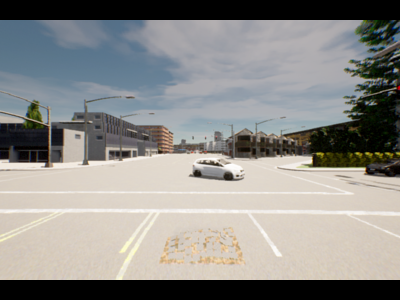
\includegraphics[trim={1.5cm 0.75cm 1.5cm 0.75cm},clip,height=0.19\textwidth]{./img/what_if/4.png}
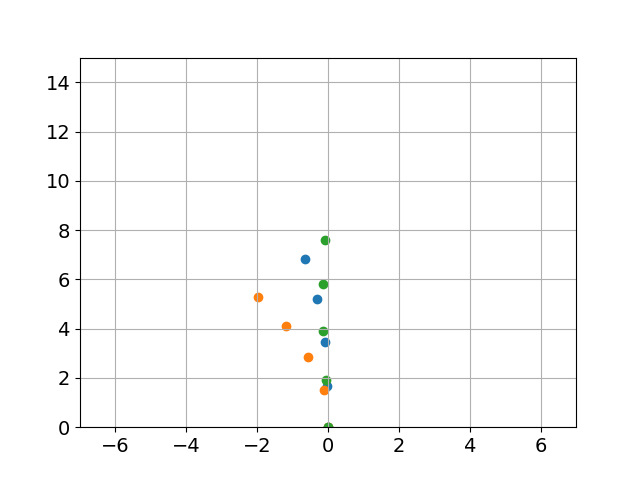
\includegraphics[trim={1cm 0.5cm 1.5cm 1cm},clip,height=0.19\textwidth]{./img/what_if/4_wp.png}
\end{center}
\vspace{-13pt}
\begin{figure}[H]
\centering
\includegraphics[height=0.01cm]{./img/deepvo_wp/1.png}
\caption{\label{fig:org01a4bfb}\textbf{``What If'' Hypothetical Pseudo-Labeling.} We generate multiple plausible future trajectories in BEV for each unlabeled frame by unformly sampling the target point location. Here we illustrate what if pseduo-labeling for two driving scenarios from our CARLA dataset.}
\end{figure}
\end{minipage} 
\subsubsection{Model Pre-Training and Fine-Tuning \label{org602bc6f}}
\label{sec:org03faa22}
As a final training step, we re-train the waypoint network \(\pi_{\vth}\) from
scratch over the large and diverse dataset \(\hat{\mathcal{D}}_{\text{SelfD}}\). The
pre-trained policy can then be further fine-tuned over the original dataset
\(\mathcal{D}\).

\subsection{OVRL: Offline Visual Representation Learning}
\label{sec:orgf5ff591}
In this section, we discuss OVRL\cite{Yadav2022}, a two-stage learning approach
proposed by Yadav et. al. and incorporate it in our autonomous driving
framework. As an overview, this learning approach includes an encoder
pretraining step using DINO, followed by downstream policy learning via behavior
cloning.
\subsubsection{Self-supervised Pretraining}
\label{sec:org5dac6c1}
As the first step, a visual encoder is pretrained using DINO \cite{Caron2021}, a
simple but effective self-supervised learning algorithm. DINO uses knowledge
distillation as a mechanism for self-training, where the student network
\(g_{\vth_{s}}\) is trained to match the output of the teacher network
\(g_{\vth_{t}}\).  As illustrated in Figure \ref{fig:orga4bf381}, it takes an input image
\(x\) and using the multi-crop strategy introduced in \cite{Caron2020}, it
generates multiple distorted views or crops from it, specifically, it produces
two global views (\(x_{1}^{g}\) and \(x_{2}^{g}\)) at \(224\times 224\) resolution
and eight local views \(x^{l}\) at a lower resolution (\(96\times 96\)). All crops
are passed through the student network while only the global views are passed
through the teacher network.  The student and teacher networks both output \(K\)
dimensional feature vectors for each view, which are converted into probability
distributions (\(P_{s}\) and \(P_{t}\)) using a temperature scaled softmax
function as follows:
\[P_{s}(x)^{(i)}=\frac{\exp\left( g_{\vth_{s}}(x)^{(i)}/\tau_{s} \right)}{\sum_{k=1}^{K}\exp\left( g_{\vth_{s}}(x)^{(k)}/\tau_{s} \right)}\]
where the temperature parameter \(\tau_{s}\) controls the sharpness of the output
distribution, and a similar formula holds for \(P_{t}\) with temperature
\(\tau_{t}\). Now, given a fixed teacher network \(g_{\vth_{t}}\), the student
network learns to match the distribution of the teacher network by minimizing
the cross-entropy loss:
\[\mathcal{L}(\vth_{s})=\sum_{x\in{x_{1}^{g},x_{2}^{g}}}\sum_{x'\in
\left\lbrace x_{1}^{g},x_{2}^{g} \right\rbrace\cup\left\lbrace x^{l}_{i} \right\rbrace_{i=1}^{8}}P_{t}(x)\log(P_{s}(x')).\] The
teacher network parameters are updated as an exponential moving average of the
student network parameters.

\begin{figure}[htbp]
\centering
\includegraphics[keepaspectratio,width=\textwidth,height=\textheight]{./img/ovrl.pdf}
\caption{\label{fig:orga4bf381}Overview of OVRL, consisting of two steps: 1) offline pretraining of the visual representations using large-scale pre-rendered images of indoor environments using DINO 2) downstream finetuning of the visuomotor representations on the ImageNav RL task in Habitat.}
\end{figure}


Representation learning by self-supervised learning algorithm is always prone to
collapse, i.e., the network can converge to a trivial solution by predicting the
same representation for every image. To avoid collapse, DINO centers and
sharpens the teacher’s output before the softmax operation. Specifically, the
centering operation adds the term \(c\) to the teacher’s output, which is
updated as follows: \(c\leftarrow mc+(1-m)\frac1B\sum_{i=0}^{B}g_{\vth_{t}}(x_{i})\),
where \(m>0\) is a momentum parameter and \(B\) is the batch size. Sharpening is
achieved by setting low value for the temperature parameter \(\tau_{t}\) for the
teacher softmax normalization. Thus, centering prevents one dimension to
dominate but encourages collapse to the uniform distribution, while the
sharpening has the opposite effect. Applying both operations balances their
effects which is sufficient to avoid collapse in presence of a momentum teacher.
\subsubsection{Implementation Details}
\label{sec:org9a9d5ac}
We use the same ResNet34 architechture as discussed in \ref{org6328e99}. We pretrain the
model on the CARLA driving scenes without the labels. We train with the AdamW
optimizer \cite{Loshchilov2017} and a batch size of 16 per-gpu, distributed over
8 GPUs. The learning rate is linearly ramped up during the first 10 epochs to
its base value determined with the following linear scaling rule
\cite{Goyal2017}: lr = 0.0005 \(\times\) batchsize/256. After this warmup, we decay the
learning rate with a cosine schedule \cite{Loshchilov2016}. The weight decay
also follows a cosine schedule from 0.04 to 0.4. The temperature \(\tau_{s}\) is
set to 0.1 while we use a linear warm-up for \(\tau_{t}\) from 0.04 to 0.07 during
the first 30 epochs. We follow the data augmentations of BYOL \cite{Grill2020}
(color jittering, Gaussian blur and solarization) and the multi-crop strategy
\cite{Caron2020}. 

\subsubsection{Downstream Learning}
\label{sec:org93ba91d}
After pre-training with DINO, the whole projection head is discarded.  Now we
plug this pre-trained ResNet34 architechture in our waypoint prediction network
(Section \ref{org6328e99}). Now this waypoint prediction network is further fine-tuned over
the small original dataset \(\mathcal{D}\). Thus, we leverage unlabeled driving scenes
to help the visual encoder attain a better representation of the input and then
we provide the network with the navigational informations through our small
original dataset \(\mathcal{D}\) and thus enables the network to quickly map the input
scenes to the waypoints leveraging the better internal representation. 

\section{Experimental Results \label{orgb8662bc}}
\label{sec:org5f9f6a1}

In this section, we provide our experimental setup, compare the driving
performance of our approach against the prior works, present an ablation study
exploring different unlabeled datasets and learning approaches and conduct an
infraction analysis to study different failure cases.

\subsection{Task}
\label{sec:org71cbfd7}
We consider the task of navigation along a set of predefined routes in a variety
of areas, e.g. freeways, urban areas, and residential districts. The routes are
defined by a sequence of sparse goal locations in GPS coordinates provided by a
global planner and the corresponding discrete navigational commands, e.g. follow
lane, turn left/right, change lane. Our approach uses only the sparse GPS
locations to drive. Each route consists of several scenarios, initialized at
predefined positions, which test the ability of the agent to handle different
kinds of adversarial situations, e.g. obstacle avoidance, unprotected turns at
intersections, vehicles running red lights, and pedestrians emerging from
occluded regions to cross the road at random locations. The agent needs to
complete the route within a specified time limit while following traffic
regulations and coping with high densities of dynamic agents. Infractions that
are penalized are:
\begin{itemize}
\item Collision with a pedestrian
\item Collision with a vehicle
\item Collision with a static object
\item Running a red light
\item Running a stop sign
\item Driving on the wrong lane or sidewalk
\item Leaving the route specified by the navigational planner
\end{itemize}
Along the routes, there are dangerous scenarios specified which the agent needs to
resolve in order to safely arrive at his destination. There are currently 10 different
scenarios specified:
\begin{itemize}
\item Rubble on the road leading to a loss of control.
\item Leading vehicle suddenly performs an emergency brake.
\item A pedestrian hidden behind a static object suddenly runs across the street.
\item After performing a turn at an intersection, a cyclist suddenly drives across
the street.
\item A slow vehicle gets spawned in front of the agent.
\item A static object is blocking the street.
\item Crossing traffic is running a red light at an intersection
\item The agent must perform an unprotected left turn at an intersection with oncoming traffic
\item The agent must perform a right turn at an intersection with crossing traffic
\item Crossing an unsignalized intersection.
\end{itemize}

\subsection{Implementation Details}
\label{sec:org201f9a4}
\subsubsection{Data Cleansing}
\label{sec:orge664fe6}
Our expert driving demostrations contain many failure cases. For examples,
ego-vehicle crashes into another vehicle or another vehicle comes infront of the
ego-vehicle while its taking a turn. For most of these failure cases, the
ego-vehicle does not move after the incident for the rest of frames in that
route demonstration. Also, in the beginning of the route demonstrations, the
ego-vehicle takes some time to reach the desired speed from zero, even though
from the BC perspective the ego-vehicle should be on full speed in such
situation as there is no car infront of it. These failure cases introduce
spurious corrections that lead to causal confusion problem
\cite{Codevilla2019}. Therefore we remove these demonstrations which leads to
improved driving performance.

\subsubsection{Stratified Sampling}
\label{sec:orgdd1802e}
On top of cleaning the data, we also group the data according to different
driving modalities. For example, dependending on the waypoints corresponding to
a driving frame, we catogorize the sample as one of the four categories --- `at
turns', `straight driving', `at halt' or `accelerating'. Next, we implement
stratified sampling technique in our dataloader, which not only use the good
samples but also generate a training batch (we use batch size of 64 in all our
experiments) consisting of equal number of examples from each modalities. We do
this because in our CARLA dataset and specifically in the YouTube dataset, we
observe that not all modalities occur equally, for example number of instances
where the car turns are very rare. This sampling technique mitigates this issue
and therefore improves the driving perfomance.

\subsubsection{Image Augmentation}
\label{sec:org0284d03}
Prior works \cite{Laskin2020,Kostrikov2020,Yarats2021,Mezghani2021} have shown
that using image augmentations during policy learning can help improve overall
performance and leads to better generalization on the test set. Even though, we
have not exhaustively searched for the optimal augmentations, but it is
intuitively understandable that heavy image augmentation will degrade driving
performance (for example, adding heavy Gaussian noise can interfere with the
traffic light signal). Thus, we use mild augmentations such that they affect
images very little. We use Gaussian noise, Gaussian blur, Dropout, Salt and
Paper noise, which lead to improved robustness of the model.

\subsection{Dataset \label{org9b7d054}}
\label{sec:org5d0a4bd}
We use the CARLA \cite{Dosovitskiy2017} simulator for training and testing,
specifically CARLA 0.9.10 which consists of 8 publicly available towns. We use 7
towns for training and hold out Town05 for evaluation. For generating training
data, we roll out an expert policy designed to drive using privileged
information from the simulation and store data at 2 FPS. We select Town05 for
evaluation due to the large diversity in drivable regions compared to other
CARLA towns, e.g. multi-lane and single-lane roads, highways and exits, bridges
and underpasses. We consider Town05-Long evaluation setting: 10 long routes of
1000-2000m comprising 10 intersections each. Each route consists of a high
density of dynamic agents and adversarial scenarios which are spawned at
predefined positions along the route. Since we focus on handling dynamic agents
and adversarial scenarios, we decouple this aspect from generalization across
weather conditions and evaluate only on ClearNoon weather.

We also use a set of first-view driving videos from YouTube collected by the
Zhang et. al. \cite{Zhang2022}. We use 52 videos with a total length of over 50
hours of driving demonstration. As shown in Figure \ref{fig:orgbcbfbbb}, these videos
cover different driving scenes with various weather conditions (sunny, rainy,
snowy, etc.) and regions (rural and urban areas). We sample two frames every one
second, resulting to a dataset of 0.36 million frames. We use all the the
YouTube driving data for pretraining the models in all learning approaches.

\subsection{Evaluation Metrics \label{orge7e1754}}
\label{sec:org6df9562}
For the CARLA Autonomous Driving Leaderboard, the driving performance of an
agent is characterized by a set of chosen metrics that considers different
aspects of driving. While all routes have the same type of metrics, their
respective values are calculated separately. These metrics are as follows:

\subsubsection{Route Completion (RC)}
\label{sec:orga4b2115}
Route Completion is the percentage of the route that is completed by an
agent. If an agent drives off-road, that percentage of the route will not be
considered towards the computation of the route completion score. Additionally,
the following events will interrupt the simulation, preventing the agent to
continue which will effectively reduce the route completion:

\begin{itemize}
\item Route deviation: If an agent deviates more than 30 meters from the assigned route.
\item Agent blocked: If an agent doesn’t take any actions for 180 simulation seconds.
\item Simulation timeout: If no client-server communication can be established in 60 seconds.
\item Route timeout: If the simulation of a route takes too long to finish.
\end{itemize}

\subsubsection{Infraction Score (IS)}
\label{sec:org2f789db}
Infraction Score is a penalty for infractions where the agent starts with
an ideal base score of 1.0. For every infraction, the score is multiplied by the
penalty coefficient of that infraction type. Ordered by their severity, the
penalty coefficients are as follows:
\begin{itemize}
\item Collision with a pedestrian: 0.50
\item Collision with a vehicle: 0.60
\item Collision with a static object: 0.65
\item Running a red light: 0.70
\item Running a stop sign: 0.80
\end{itemize}
Note that this means that subsequent infractions will have a lower impact due to the
multiplicative nature of the score.

\subsubsection{Driving Score (DS)}
\label{sec:orgbf0416f}
Driving Score is the main metric for performance, serving as the product between
the route completion and the infractions penalty. It is calculated in the
following way: \[\text{Driving Score}=\frac1N\sum_{i=1}^{N}R_{i}P_{i}\] where \(N\) is the
number of routes, \(R_{i}\) the route completion percentage of the \(i\)-th route and
\(P_{i}\) the infraction penalty of \(i\)-th route. Note that, this is not the
same as multiplying the averaged route completion with the averaged infraction
score. The driving score is a normalized metric, meaning that the best possible
score is 100 and the worst score is 0. For the validation routes, we run them
with 3 different seeds and report the mean and standard deviation of the 3
scores averaged across the routes.

\subsection{Results}
\label{sec:org4273f08}

\subsubsection{Performance of Supervised Training}
\label{sec:org07d94be}

\begin{table}
\begin{longtable}{|r|r|r|r|r|r|}
\hline
\raggedleft {\bfseries ImgAug} &
\raggedleft {\bfseries \(\begin{matrix*}[r] \textbf{Cleaned Data} \\ \textbf{+ Stratified Sampling} \end{matrix*}\)} &
\raggedleft {\bfseries lr} &
\raggedleft {\bfseries DS \((\uparrow)\)} &
\raggedleft {\bfseries RC \((\uparrow)\)} &
\raggedleft\arraybslash {\bfseries IS \((\uparrow)\)}\\\hline
\raggedleft \xmark &
\raggedleft \xmark &
\raggedleft 1e-4 &
\raggedleft 13.39 {\textpm} 1.81 &
\raggedleft 60.31 {\textpm} 6.11 &
\raggedleft\arraybslash 0.35 {\textpm} 0.02\\
\raggedleft \xmark &
\raggedleft \xmark &
\raggedleft 2e-5 &
\raggedleft 17.57 {\textpm} 3.34 &
\raggedleft 68.75 {\textpm} 5.70 &
\raggedleft\arraybslash 0.32 {\textpm} 0.04\\
\raggedleft \xmark &
\raggedleft \cmark &
\raggedleft 2e-5 &
\raggedleft 20.91 {\textpm} 2.83 &
\raggedleft 71.26 {\textpm} 4.84 &
\raggedleft\arraybslash 0.34 {\textpm} 0.01\\
\raggedleft \cmark &
\raggedleft \xmark &
\raggedleft 2e-5 &
\raggedleft 28.55 {\textpm} 3.92 &
\raggedleft 85.47 {\textpm} 9.23 &
\raggedleft\arraybslash 0.36 {\textpm} 0.07\\
\raggedleft \cmark &
\raggedleft \cmark &
\raggedleft 2e-5 &
\raggedleft{\bfseries 32.24 {\textpm} 4.72} &
\raggedleft{\bfseries 91.92 {\textpm} 8.01} &
\raggedleft\arraybslash{\bfseries 0.37 {\textpm} 0.05}\\\hline
\caption{Results on the NEAT evaluation routes for a fully supervised sensorimotor agent (AIM) trained with various adhoc techniques}
\label{table2}
\end{longtable}
\end{table}


In our first experiment, we examine to what extent we can improve the current
image-based AIM architechture \cite{Prakash2021} in CARLA evaluation setting
involving complex multi-lane intersections, adversarial scenarios, and heavy
infraction penalties. In Table \ref{table2}, we report the evaluation results of
supervised training with all the 7 CARLA training towns (Section \ref{org9b7d054}) over 3
random seeds. We observe that smaller learning rate improve the driving
performance. Next, we train the model with the filtered data and train with
stratified sampling enabled dataloader. Here again we get an improvement in
driving performance by a small margin. Lastly, we introduce image augmentation
in our training. We find that image augmentation helps improve the performance
by a large margin. We note that each of these techniques improve the driving
independently. Thus, combining all these techniques, we gain significant improve
in the driving perfomance cumulating their individual contributions.

\subsubsection{Perfomance of the Learning Approaches}
\label{sec:org87447f2}
For all our semi-supervised and self-supervised learning approaches, we consider
demonstrations from Town 1 and Town 2, as our small dataset \(\mathcal{D}\) with
ground-truth labels. We consider driving scenes from rest of the towns as our
unlabeled dataset \(\mathcal{U}_{\text{CARLA}}\). We also form an unlabeled dataset
\(\mathcal{U}_{\text{YouTube}}\) containing driving scenes from YouTube videos and
combining these two dataset we have the unlabeled dataset \(\mathcal{U}_{\text{CARLA +
YouTube}}\). We consider various approaches for leveraging the unlabeled CARLA
and YouTube data. To emphasize generalization, we do not pseudo-label the unseen
test datasets or incorporate their unlabeled samples into the self-training in
any way. We incorporate the same adhoc techniques in the self-training that
improved performance in full supervised training. We report the closed-loop
evaluation performance on Town05 long routes for all tests in Table
\ref{table3}.
\begin{table}
{\footnotesize
\begin{longtable}{|l|l|r|r|r|}
\hline
{\bfseries Datasets} &
{\bfseries Method} &
\raggedleft{\bfseries DS \((\uparrow)\)} &
\raggedleft{\bfseries RC \((\uparrow)\)} &
\raggedleft\arraybslash{\bfseries IS \((\uparrow)\)}\\\hline
Labeled Dataset: \(\mathcal{D}\) &
AIM (w/o confidence) &
\raggedleft 7.83 {\textpm} 0.56 &
\raggedleft 51.01 {\textpm} 4.68 &
\raggedleft\arraybslash 0.32 {\textpm} 0.03\\\hhline{~----}
~
 &
AIM (w/ confidence) &
\raggedleft 5.97 {\textpm} 0.78 &
\raggedleft 54.35 {\textpm} 5.88 &
\raggedleft\arraybslash 0.19 {\textpm} 0.02\\\hline
Unlabeled Datasets: \(\mathcal{U}_{\text{CARLA}}\) &
SelfD (w/o What If, w/o confidence) &
\raggedleft 6.07 {\textpm} 0.41 &
\raggedleft 58.36 {\textpm} 3.08 &
\raggedleft\arraybslash 0.17 {\textpm} 0.02\\\hhline{~----}
Labeled Dataset: \(\mathcal{D}\) &
SelfD (w/o What If, w/ confidence) &
\raggedleft 8.3 {\textpm} 2.75 &
\raggedleft 59.89 {\textpm} 9.87 &
\raggedleft\arraybslash 0.22 {\textpm} 0.03\\\hhline{~----}
~
 &
SelfD (w/ What If, w/o confidence) &
\raggedleft 5.02 {\textpm} 0.51 &
\raggedleft 53.32 {\textpm} 3.98 &
\raggedleft\arraybslash 0.18 {\textpm} 0.01\\\hhline{~----}
~
 &
SelfD (w/ What If, w/ confidence) &
\raggedleft 4.67 {\textpm} 0.86 &
\raggedleft 49.15 {\textpm} 6.43 &
\raggedleft\arraybslash 0.15 {\textpm} 0.02\\\hhline{~----}
~
 &
SemiD (transductive training) &
\raggedleft{\bfseries 13.25 {\textpm} 2.55} &
\raggedleft{\bfseries 95.06 {\textpm} 5.33} &
\raggedleft\arraybslash{\bfseries 0.13 {\textpm} 0.02}\\\hhline{~----}
~
 &
SemiD (finetuned) &
\raggedleft 12.58 {\textpm} 0.32 &
\raggedleft 90.88 {\textpm} 3.91 &
\raggedleft\arraybslash 0.14 {\textpm} 0.02\\\hline
Unlabeled Datasets: \(\mathcal{U}_{\text{CARLA + YouTube}}\) &
SelfD (w/o What If, w/o confidence) &
\raggedleft 6.66 {\textpm} 1.98 &
\raggedleft 51.44 {\textpm} 7.23 &
\raggedleft\arraybslash 0.23 {\textpm} 0.03\\\hhline{~----}
Labeled Dataset: \(\mathcal{D}\) &
SelfD (w/o What If, w/ confidence) &
\raggedleft 5.17 {\textpm} 1.59 &
\raggedleft 55.46 {\textpm} 8.57 &
\raggedleft\arraybslash 0.16 {\textpm} 0.05\\\hhline{~----}
~
 &
SelfD (w/ What If, w/o confidence) &
\raggedleft 7.28 {\textpm} 0.65 &
\raggedleft 47.21 {\textpm} 5.03 &
\raggedleft\arraybslash 0.26 {\textpm} 0.02\\\hhline{~----}
~
 &
SelfD (w/ What If, w/ confidence) &
\raggedleft 6.22 {\textpm} 1.12 &
\raggedleft 51.34 {\textpm} 6.8 &
\raggedleft\arraybslash 0.21 {\textpm} 0.03\\\hhline{~----}
~
 &
SemiD (transductive training) &
\raggedleft 8.87 {\textpm} 2.01 &
\raggedleft 92.93 {\textpm} 6.77 &
\raggedleft\arraybslash 0.11 {\textpm} 0.03\\\hhline{~----}
~
 &
SemiD (finetuned) &
\raggedleft 10.15 {\textpm} 1.23 &
\raggedleft 93.38 {\textpm} 6.31 &
\raggedleft\arraybslash 0.1 {\textpm} 0.01\\\hhline{~----}
~
 &
OVRL &
\raggedleft 7.78 {\textpm} 1.26 &
\raggedleft 83.13 {\textpm} 7.78 &
\raggedleft\arraybslash 0.12 {\textpm} 0.04\\\hhline{~----}
~
 &
OVRL + SemiD (transductive training) &
\raggedleft 5.51 {\textpm} 2.26 &
\raggedleft{\bfseries 97.54 {\textpm} 2.74} &
\raggedleft\arraybslash 0.06 {\textpm} 0.02\\\hhline{~----}
~
 &
OVRL + SemiD (finetuned) &
\raggedleft 9.79 {\textpm} 1.22 &
\raggedleft 90.66 {\textpm} 0.29 &
\raggedleft\arraybslash 0.14 {\textpm} 0.01\\\hline
Unlabeled Datasets: \(\mathcal{U}_{\text{YouTube}}\) &
SemiD (transductive training) &
\raggedleft{\bfseries {}-} &
\raggedleft{\bfseries {}-} &
\raggedleft\arraybslash{\bfseries {}-}\\\hhline{~----}
Labeled Dataset: \(\mathcal{D}\) &
SemiD (finetuned) &
\raggedleft {}- &
\raggedleft {}- &
\raggedleft\arraybslash {}-\\\hline
\caption{Results on the NEAT evaluation routes for sensorimotor agent (AIM) trained with various semi-supervised and self-supervised learning approaches}
\label{table3}
\end{longtable}
}
\end{table}

\textbf{Baselines:} The first two rows of Table \ref{table3} shows evaluation scores of the AIM
baseline trained supervisedly on Town 1 and 2. We report evaluation on two
models with same internal specification and only differ in the outputs --- one
predicts the waypoints and the other one predicts confidence score in addition
to the waypoints.

\textbf{SelfD:} Table \ref{table3} also shows results of SelfD with or without ``What If''
augmentation and confidence prediction in all combinations, for two unlabeled
datasets \(\mathcal{U}_{\text{CARLA}}\) and \(\mathcal{U}_{\text{CARLA + YouTube}}\). But, we see no
noticeable improvement and even reduction in perfomance in the evaluations
compared to supervised training on Town1\&2. SelfD training without ``What If''
augmentation on \(\mathcal{U}_{\text{CARLA}}\) dataset shows very small improvement in the
route completion, but this can also be accounted for noise in the
evaluation. Thus, contrary to the claim by the authors of SelfD
\cite{Zhang2022a}, we observe that SelfD gains no generalization with ``What
If'' augmentation. Figure \ref{fig:orgbb6bff0} demonstrates some of the cases where
SelfD fails to produce appropriate pseduo-waypoints, but SemiD produces the
correct ones.

\afterpage{\vspace*{\fill}
\begin{minipage}{\textwidth} 
\begin{center}
\includegraphics[trim={1.5cm 0.75cm 1.5cm 0.75cm},clip,height=0.19\textwidth]{./img/compare/7.png}
\includegraphics[trim={1cm 0.5cm 1.5cm 1cm},clip,height=0.19\textwidth]{./img/compare/7_wp.png}
\hfill
\includegraphics[trim={1.5cm 0.75cm 1.5cm 0.75cm},clip,height=0.19\textwidth]{./img/compare/8.png}
\includegraphics[trim={1cm 0.5cm 1.5cm 1cm},clip,height=0.19\textwidth]{./img/compare/8_wp.png}

\hspace{0.19\textwidth} (a) \hfill (b) \hspace{0.19\textwidth}
\vspace{5pt}

\includegraphics[trim={1.5cm 0.75cm 1.5cm 0.75cm},clip,height=0.19\textwidth]{./img/compare/9.png}
\includegraphics[trim={1cm 0.5cm 1.5cm 1cm},clip,height=0.19\textwidth]{./img/compare/9_wp.png}
\hfill
\includegraphics[trim={1.5cm 0.75cm 1.5cm 0.75cm},clip,height=0.19\textwidth]{./img/compare/10.png}
\includegraphics[trim={1cm 0.5cm 1.5cm 1cm},clip,height=0.19\textwidth]{./img/compare/10_wp.png}

\hspace{0.19\textwidth} (c) \hfill (d) \hspace{0.19\textwidth}
\vspace{5pt}

\includegraphics[trim={1.5cm 0.75cm 1.5cm 0.75cm},clip,height=0.19\textwidth]{./img/compare/12.png}
\includegraphics[trim={1cm 0.5cm 1.5cm 1cm},clip,height=0.19\textwidth]{./img/compare/12_wp.png}
\hfill
\includegraphics[trim={1.5cm 0.75cm 1.5cm 0.75cm},clip,height=0.19\textwidth]{./img/compare/11.png}
\includegraphics[trim={1cm 0.5cm 1.5cm 1cm},clip,height=0.19\textwidth]{./img/compare/11_wp.png}

\hspace{0.19\textwidth} (e) \hfill (f) \hspace{0.19\textwidth}
\vspace{5pt}

\includegraphics[trim={1.5cm 0.75cm 1.5cm 0.75cm},clip,height=0.19\textwidth]{./img/compare/13.png}
\includegraphics[trim={1cm 0.5cm 1.5cm 1cm},clip,height=0.19\textwidth]{./img/compare/13_wp.png}
\hfill
\includegraphics[trim={1.5cm 0.75cm 1.5cm 0.75cm},clip,height=0.19\textwidth]{./img/compare/14.png}
\includegraphics[trim={1cm 0.5cm 1.5cm 1cm},clip,height=0.19\textwidth]{./img/compare/14_wp.png}

\hspace{0.19\textwidth} (g) \hfill (h) \hspace{0.19\textwidth}\(\,\)
\end{center}
\vspace{-13pt}
\begin{figure}[H]
\centering
\includegraphics[height=0.01cm]{./img/deepvo_wp/1.png}
\caption{\label{fig:orgbb6bff0}Some failure cases where SelfD could not recover the desired pseduo-waypoints but correctly recovered by DeepVO. Examples (a), (b), (c), show some situations where the ego-vehicle should moves forward but SelfD predicts waypoints to slow down the ego-vehicle. Examples (d), (e) show situations where ego-vehicle should not move because of the cyclist infront or the crossing vehicles, but in this case SelfD predicts waypoints to keep the ego-vehicle moving. Examples (f), (g), (h), show situations where the ego-vehicle should stop because of the red-light, yet SelfD predicts waypoints violating the red-light stop.}
\end{figure}
\end{minipage} 
\vspace*{\fill}\clearpage}


\textbf{SemiD:} We train our DeepVo architechture with Town1\&2 data containing driving
scenes and its corresponding ego-vehicle positions and gather pseduo-waypoints
and pseudo-target-point for all the unlabeled dataset. We report results of
SemiD for three unlabled dataset \(\mathcal{U}_{\text{CARLA}}\), \(\mathcal{U}_{\text{YouTube}}\)
and \(\mathcal{U}_{\text{CARLA + YouTube}}\) in Table \ref{table3}. Contrary to the claim
by the authors of SelfD \cite{Zhang2022a}, we observe this method improve
driving perfomance by a huge margin. With only transductive learning stage
(i.e. training with pseduo-labels) of semi-supervised learning, we achieve a
near doubling score in driving score (DS) and route completion (RC), from 7.83
to 13.25 in driving score and 51\% to 95\% in route completion. We observe this
performance improvement across all unlabeled datasets. We note that while our
supervised AIM Baseline benefits from the known fixed perspective transform
assumption, SemiD does not incorporate any knowledge of camera parameters and
must learn it from the data, yet SemiD achieves comparable perfomance in route
completion as fully supervisedly trained model on all CARLA training towns (see
Table \ref{table2}).

\textbf{OVRL:} We also shows perfomance of the self-supervised learning approach OVRL
Table \ref{table3}. We pre-train the ResNet34 backbone on the \(\mathcal{U}_{\text{CARLA +
YouTube}}\) unlabeled dataset self-supervisedly and fine-tuned on Town1\&2. Here
also we gain improvement in driving score from 51\% to 83\%. We also combine OVRL
and SemiD, by using the pretrained ResNet backbone from OVRL in SemiD. In this
case, we achieve further improvement in driving performance (97.5\% in RC with
less variance) which surpasses the avgerage route completion achieved by
supervisedly trained model on all CARLA training towns and after finetuning on
the Town1\&2, we achieve better infraction score and thus better driving score.

\textbf{Limitations:} Even though, in all of these learning approaches we achieve near
perfect route completion, we can observe that we do not gain improvement in
infraction score. The reason is two fold. Firstly, since the driving agent now
covers on average more than 90\% of the routes, the total number of infractions
also increases compared to when the agent covers 50\% of the routes (as for AIM
Baseline) and because of the multiplicative nature of the infraction score
metric, the infraction score and driving score is very much affected. Secondly,
in both SelfD and SemiD, the generated pseduo-waypoints are noisy especially
when the ego-vehicle stands still and therefore it is hard for the the model map
appropriate behavior in all infraction scenarios and for OVRL it happens because
the traffic light signal in the european towns is significantly different from
the evaluation town which has the highway traffic lights. Beyond these reasons,
infractions due to invisibilty (e.g. the highway traffic light is not visible or
ego-vehicle changes lane but the rear vehicle collide with it or the passenger
starts walking after the car already have gone past it) is one of the biggest
reason why infraction score is affected even in supervised training.

\section{Conclusion \label{org156c67e}}
\label{sec:org34f091b}

In this thesis, we proposed, SemiD, a novel semi-supervised learning approach
based on deep visual odometry. We have also explored some prior works in our
autonomous driving framework that use semi-supervised and self-supervised
learning for navigation, namely `SelfD' and `OVRL'. We showed that SemiD
outperforms the prior works on the challenging NEAT evaluation routes by
achieving 95\% in RC. We also observed that OVRL can learn generalizable
representations and bring substantial improvement in driving perfomance with
97.5\% in RC when combined with SemiD. Thus, we showed that we can significantly
improve perfomance of a self-driving agent without incurring additional data
collection or annotation efforts, i.e., for a new platform, perspective,
use-case, or ambient settings. We also showed that our model architechture can
learn how to maneuver in diverse driving situations in different camera
configurations. Thus, we envision that the proposed approach can be leveraged in
real-world generalization and adaptation settings for autonomous driving
systems.


Even though SemiD achieved almost perfect route completion, it incurred
infraction frequently. Thus, a future direction could be to investigate this
issue. Also our model development was restricted to large-scale training with
single frame. Therefore it would be interesting to study if this method can gain
benefit from temporal demonstrations. Finally, beyond complex 3D navigation, it
would be interesting to explore the applicability of our proposed training
framework for learning various embodied tasks from unlabeled web data.


\printbibliography
\end{document}